\section{Caractérisation et analyse de performance des architectures}
\label{chap:performance} \label{sec:edl_perf_intro}

    Dans la section précédente, nous avons discuté des différentes opportunités disponibles pour permettre la construction de plateformes \gls{exascale}. De nouvelles technologies comme les mémoires SCM ou la photonique vont permettre de développer de nouvelles architectures. Grâce au protocole Gen-Z, différentes architectures pourront facilement être interconnectées dans une même plateforme. L'efficacité énergétique étant primordiale, il est fondamental de trouver les architectures les plus adaptées pour chaque application et d'optimiser leur code pour en tirer la performance maximale. Nous proposons ainsi d'étudier deux domaines permettant de réaliser ce travail: le domaine de la caractérisation d'architecture et le domaine du suivi de performance. 
    
    La \autoref{sec:caracterisation} présente les méthodes et les outils existants permettant de caractériser les matériels. Dans un supercalculateur, de nombreuses ressources doivent être caractérisées: le processeur, le système d'interconnexion, le système de stockage... 
    Dans ce travail de thèse, nous nous sommes principalement intéressés à la caractérisation de la microarchitecture des processeurs et du système mémoire:
    \begin{itemize}
        \item Les applications \gls{HPC} utilisent ces architectures pour exécuter des opérations sur des nombres à virgule flottante (\gls{FLOP}). Nous nous intéressons donc au matériel responsable de leur exécution: les unités arithmétiques et logiques (ALU).
        
        \item La performance de la majorité des applications étant limitée par le système mémoire, nous nous intéresserons dans un second temps à la caractérisation du système mémoire. Ce dernier étant composé d'une hiérarchie de différentes mémoires, il est important de pouvoir caractériser ses différents niveaux: taille, latence, débit.
    \end{itemize}
    
    La \autoref{sec:profiling} présente les méthodes et les outils existants permettant de suivre les performances des applications. La complexité des architectures et la différence d'évolution des performances du système mémoire et des processeurs empêchent les applications d'atteindre les performances maximales délivrées par les processeurs. 
    \begin{itemize}
        \item Le temps d'exécution des applications HPC est généralement passé dans une faible portion des lignes de codes. Ces zones, appelées \glspl{hotspot}, doivent être identifiées pour être caractérisées et optimisées. Pour cela, le programmeur doit utiliser des outils permettant d'obtenir les profils de performances d'une application et identifier ces zones de codes.
        
        \item Il est ensuite nécessaire de pouvoir mesurer la performance effective de ces zones de code. Lorsque la performance maximale n'est pas atteinte, il est alors nécessaire de pouvoir en expliquer les raisons. 
    \end{itemize}
    
      
\subsection{Caractérisation des architectures}\label{sec:caracterisation}
%%%%%%%%%%%%%%%%%%%%%%%%%%%%%%%%%%%%%%%%%%%%%%%%%%%%%%%%%%%%%%%%%%%%%%%%
%%%%%%%%%%%%%%%%%%%%%%%%%%%%%%%%%%%%%%%%%%%%%%%%%%%%%%%%%%%%%%%%%%%%%%%%
    
    Dans cette partie, nous présentons les différentes méthodes permettant de caractériser les architectures. Nous utilisons le terme \textit{caractérisation} pour désigner la capacité à identifier les forces et les faiblesses d'une architecture ainsi que d'en mesurer certaines caractéristiques. Afin de choisir la meilleure architecture pour une application il est nécessaire de connaître ces différentes caractéristiques: capacité de calcul, performance mémoire (débit, latence)...
    
    Il existe deux façons de caractériser une architecture: 
    \begin{itemize}
        \item La première consiste à utiliser les données communiquées par le constructeur d'une plateforme pour calculer la performance du matériel. Dans la \autoref{sec:methodo_step1} nous montrons comment le débit mémoire et la performance de calcul théoriques peuvent être calculés à partir des documentations techniques. Cette approche est intéressante, car elle permet de caractériser une architecture sans y avoir accès. Cependant, certaines données peuvent ne pas être disponibles et nécessitent d'avoir accès aux architectures pour les obtenir. Des outils disponibles sur les distributions Linux (\textit{lscpu\footnote{\url{http://man7.org/linux/man-pages/man1/lscpu.1.html}}, cpumap\footnote{\url{https://www.plafrim.fr/fr/outils-sgi/}}, cpuid\footnote{\url{https://www.felixcloutier.com/x86/cpuid}}}) peuvent alors être utilisées pour les obtenir. Néanmoins, ces outils peuvent ne pas supporter toutes les architectures et certaines données peuvent manquer.
    
        \item La seconde méthode nécessite d'avoir accès à l'architecture dans le but d'y exécuter des codes dont l'objectif est de mesurer la performance. Ces codes, appelés \glspl{benchmark}, sont présentés dans la section suivante. Contrairement à la première méthode, l'utilisation de ces applicatifs permet de mesurer une performance réellement atteignable (performance crête). En effet, il est rare que la performance mesurée soit égale à la performance théorique calculée à partir des données techniques de l'architecture. Le développement de nouvelles architectures, et la complexité de leur microarchitecture peuvent donner lieu à des bogues et conduire à de mauvaises performances. Il est donc important de les caractériser pour identifier une erreur, mais aussi pour comparer la performance d'une application avec la performance réelle de l'architecture.
    \end{itemize}
    
           
    \subsubsection{Benchmarks}
    %%%%%%%%%%%%%%%%%%%%%%%%%%%%%%%%%
           
        En informatique, un \gls{benchmark} est un code, ou un ensemble de codes, permettant de mesurer la performance d'une solution et d'en vérifier ses fonctionnalités. Lors de la phase de conception d'une architecture, des benchmarks peuvent être utilisés pour détecter la présence de bogues ou pour valider certaines fonctionnalités. Cela permet d'estimer la performance d'un matériel avant qu'il ne soit produit (grâce à des simulateurs par exemple). Les codes de benchmark sont pour la majorité en version libre de droits. Cela permet leur large utilisation et permet de comparer la performance de différentes plateformes (le classement du Top500 est réalisé grâce au benchmark HPL). En informatique, nous pouvons classer les benchmarks selon quatre catégories \cite{Staelin2004}:
        
        \begin{enumerate}

            \item  \textbf{Les benchmarks} sont des applications complètes exécutant différents types d'instructions: calculs, transferts mémoires, réseaux... Il peut aussi arriver que des applications réelles soient finalement utilisées comme programme de benchmark tel que BSMBench \cite{HPC:bsmbench} utilisé pour réaliser des motifs de calculs similaires à ceux réalisées en théorie de jauge (physique des particules). \textbf{TODO reprendre}
        
            \item  \textbf{Les benchmarks noyaux} (\textit{kernel-based benchmark}) sont des codes simples permettant de caractériser une partie spécifique du matériel. Ces codes artificiels peuvent être de simples extraits de benchmark. Le benchmark noyaux STREAM \textbf{todo citation} consiste en l'exécution de quatre fonctions différentes qui à l'origine étaient utilisées pour étudier les différences de performances entre deux architectures pour exécuter des applications pour la modélisation du climat. Il est aujourd'hui utilisé pour mesurer le débit mémoire atteignable par un processeur.
        
            \item \textbf{Les micro benchmarks} sont des benchmarks noyaux permettant d’isoler une partie précise de l’architecture à évaluer. Par exemple, lmbench \cite{HPC:lmbench} est une suite de micro benchmarks portables utilisés pour mesurer des caractéristiques importantes de la mémoire telles que la bande passante, la latence mémoire et les performances des différents niveaux de cache.  Les informations récupérées permettent de mettre en oeuvre des optimisations en s'adaptant parfaitement aux caractéristiques d'une architecture.
      
            \item \textbf{Les générateurs de benchmarks} permettent de produire une application à partir d'un premier code. La génération a l'avantage de faciliter le test de plusieurs configurations différentes en faisant varier les paramètres d'entrée, la taille des jeux de données, ou encore l'algorithme utilisé pour résoudre une tâche. Ainsi, le logiciel de GeneNetWeaver \cite{schaffter2011genenetweaver} peut être utilisé pour générer dynamiquement des modèles génétiques pouvant ensuite être utilisés comme benchmark. Des bibliothèques de calcul telles que ATLAS \cite{whaley1998automatically} et FFTW \cite{frigo1998fftw} génèrent des micro benchmarks pour caractériser l'architecture. ATLAS génère ainsi des dizaines de versions différentes d'un code de multiplication de matrices pour estimer la taille de bloc la plus efficace pour exploiter les caches.
        \end{enumerate}    
   
     
    \subsubsection{Benchmarks existants}
    %%%%%%%%%%%%%%%%%%%%%%%%%%%%%%%%%

        Comme indiqué dans l'introduction de cette section, nous nous sommes intéressés à la caractérisation du système mémoire ainsi qu'à celle des unités arithmétiques et logiques des processeurs. Ces unités sont responsables de l'exécution des instructions de calcul sur nombre à virgule flottante (FLOP). Elles sont donc un matériel essentiel des architectures pour l'exécution d'application de calcul intensif. Le système mémoire étant le goulot d'étranglement de la performance d'une majorité d'applications, de nombreux travaux ont été réalisés pour sa caractérisation et son optimisation. Dans cette partie nous énumérons et discutons les principaux benchmarks permettant de caractériser ces parties de l'architecture.


        %Il existe de nombreux benchmarks permettant de caractériser différentes parties du système mémoire: les accès mémoires concurrents de systèmes multiprocesseurs\cite{Mandal2010}, polices de mappage mémoire des systèmes NUMA \cite{Diener2015}, prédiction de la bande passante mémoire en fonction du placement des coeurs \cite{Wang2016a}, caractérisation de la hiérarchie mémoire \cite{Cooper2011}.
 
        

        \paragraph{HPL \cite{Dongarra2003}} 
            Un des micros benchmarks les plus utilisés est sans doute celui du HPL, utilisé pour construire le classement du Top500 \cite{HPC:top500}. Les premières versions du benchmark, alors appelé LINPACK, remontent aux années 1979 et permettaient d'estimer le temps de résolution d'un problème d'algèbre. Son utilisation comme benchmark est plus un accident qu'une réelle volonté. L'annexe B du manuel de l'utilisateur proposait aux utilisateurs d'estimer et de noter les temps de résolution en fonction de la machine utilisée. Pour pouvoir être utilisé sur les supercalculateurs, le benchmark a été parallélisé, changeant ainsi de nom en Highly Parallel Computing Benchmark, HPLinpack ou encore HPL. Il est utilisé pour mesurer le nombre maximum d'opérations à virgule flottante par seconde (\gls{FLOPS}) qu'un supercalculateur est capable de fournir pour la résolution d'un système linéaire d'équations utilisant la décomposition LU. Ainsi, avant d'être un benchmark de processeur, c'est un benchmark de librairie DGEMM (Intel MKL, netlib, GotoBLAS). La force de ce benchmark est de n'avoir qu'un résultat (soit la sommation des puissances de calculs de tous les coeurs utilisés). Il est donc très facile de comparer deux plateformes de calculs. Bien que mondialement utilisé, le HPL a un principal défaut qui est d'estimer la performance d'une plateforme en ne mesurant que sa capacité de calcul. Cependant, comme nous l'avons montré précédemment, la performance de la majorité des applications est limitée par la performance de la bande passante. La mesure du HPL n'est donc pas la plus représentative de la puissance d'un supercalculateur atteignable par des applications réelles. 
        
        \paragraph{HPCG \cite{Dongarra2013}} 
        \label{sec:hpcg}
            
            Admettant la faiblesse du benchmark HPL, son concepteur, Jack Dongarra, se mit à la recherche d'un ou d'un ensemble de benchmarks permettant de mieux caractériser ces plateformes. Avec Michael Heroux et Piotr Luszczek, ils ont présentèrent alors en 2015 le benchmark HPCG (high performance conjugate gradient). HPCG permet de couvrir de nombreux motifs de communication (globale et voisinage) et de calculs  (mis-à jour de vecteur, multiplication de matrices creuses). 
            Le premier prérequis était alors de pouvoir produire, grâce à ce nouveau benchmark, un classement des supercalculateurs représentatif de leur performance pour exécuter des applications réelles. Le deuxième prérequis fait suite à la crainte de voir la conception des processeurs être influencée pour obtenir de meilleures performances pour le benchmark HPL \cite{Dongarra2013}. Ainsi, HPCG utilise une mesure qui pousserait les concepteurs de processeurs à améliorer leurs matériels ce qui par conséquent profiterait aux applications réelles. \textbf{todo relire les temps de cette phrase avant} Là où HPL ne fournit qu'un seul résultat par exécution, HPCG en présente 128. Le classement du Top500 est aujourd'hui publié avec les valeurs obtenues par HPL et par HPCG\footnote{Classement HPCG 2019: \url{https://www.hpcg-benchmark.org/custom/index.html?lid=155&slid=302}}. Malgré la meilleure adéquation de HPCG à caractériser les plateformes, le benchmark HPL est, et sera probablement toujours utilisé, principalement pour des raisons d'historiques. En effet, il permet de suivre l'évolution des architectures depuis plus de 25 ans. 
            
        \paragraph{HPCC \cite{Luszczek2006}} 
            
            La suite de benchmark HPC Challenge vient compléter le benchmark HPL avec 6 codes dont certains réalisent des accès aux données permettant aussi de caractériser le système mémoire (voir \autoref{pic_bench_hpcc}). La suite de benchmarks est ainsi composée de HPL, Stream, DGEMM, RandomAccess, b\_eff, PTRANS, FFT. Avec l'ajout de ces six autres codes, la suite HPCC est plus représentative des applications réelles. Ces codes existaient avant la création de la suite HPCC. Le travail réalisé a permis de les regrouper dans une même suite, et de les améliorer avec des systèmes de vérifications et de rapport. Une fois compilé, un seul programme exécutable est généré permettant de faciliter son usage avec un gestionnaire de \textit{job}. Un seul exécutable étant généré, l'environnement d'exécution est le même pour tous les benchmarks de la suite (pas d'optimisation de pages larges pour un seul benchmark de la suite). 
            
            \begin{figure}
                \center
                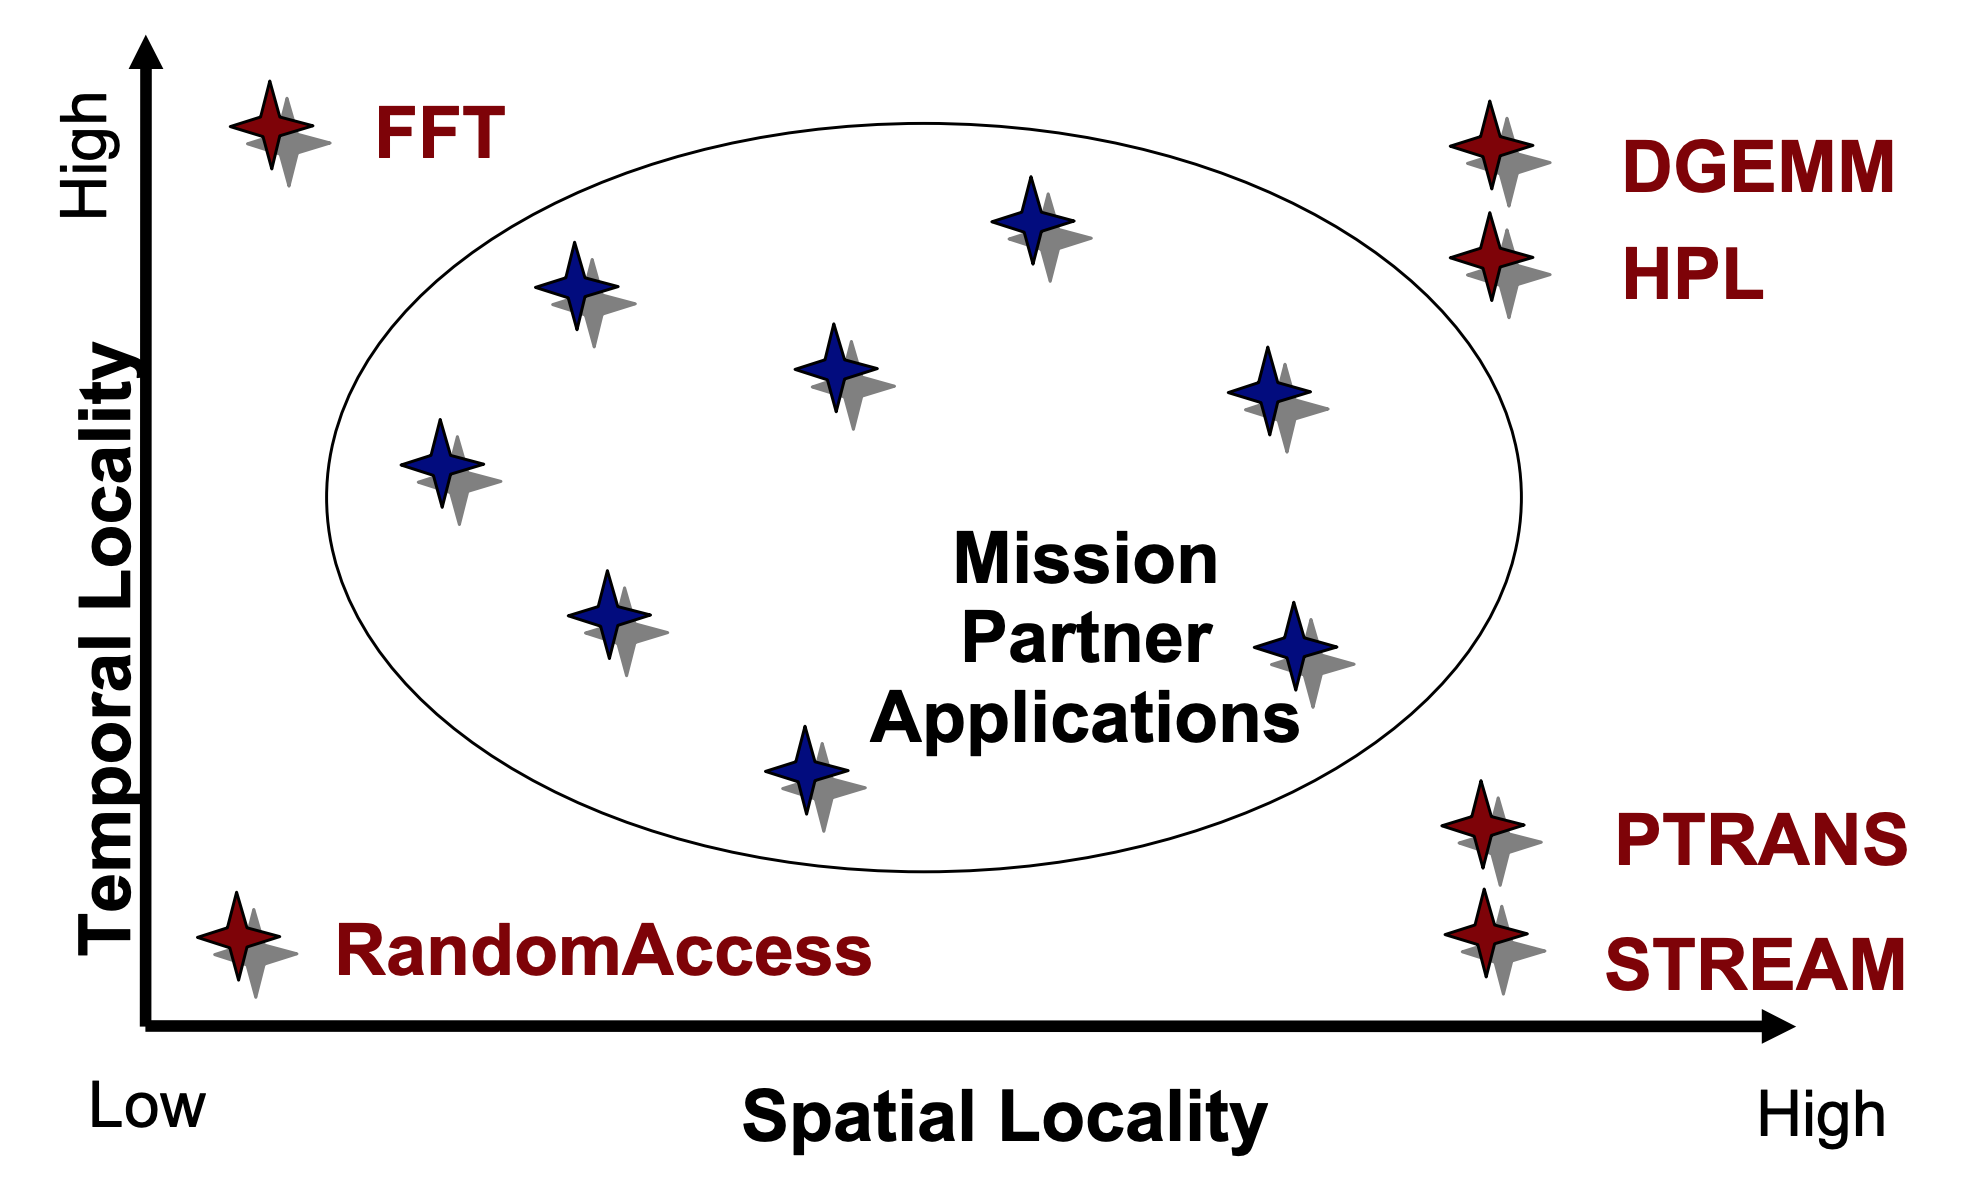
\includegraphics[width=10cm]{images/bench_hpcc.png}
                \caption{ La suite de benchmark HPCC utilise des codes utilisant des localités différentes permettant de mieux caractériser les architectures
                \label{pic_bench_hpcc}}
            \end{figure}
        
        
        \paragraph{SPEC CPU2017 \cite{Bucek2018}} 
        
            Cette nouvelle génération de benchmark produite par SPEC (Standard Performance Evaluation Corporation) qui fait suite à la version précédente SPEC CPU2006. Ces deux initiatives ont permis de regrouper des applications réelles de tailles différentes, mais dont les performances sont limitées par la puissance de calcul de l'architecture. Les applications sélectionnées sont facilement portables. La première version contenait deux suites de benchmarks (CINT2006 \cite{Dilipbhai2012} et CFP2006 \cite{Sharkawi2009}) permettant de mesurer et comparer les performances de calculs en utilisant des opérations entières ou à nombres flottants. L'objectif principal de ces codes était alors de caractériser les performances du processeur, de la hiérarchie mémoire et du compilateur. La version 2017 possède 43 benchmarks qui sont portés sur plusieurs architectures dont AMD64, Intel IA32, Power ISA ou SPARC. Les benchmarks sont organisés en quatre suites permettant de mesurer le débit et la vitesse d'exécution d'opérations utilisant des nombres entiers ou flottants.  Les différents benchmarks ont un domaine d'application spécifique (compression vidéo, rendu 3D...) et peuvent être utilisés pour la conception de processeurs optimisés pour ces charges de travail \cite{Panda2018}. Malheureusement le prix de ces benchmarks avoisine les 1000\$. Cependant les nombreux résultats, libres de droits, sont publiés leur site internet. 
        
      %  \paragraph{SHOC \cite{danalis2010scalable}.} 
            %Les plateformes HPC modernes deviennent toujours plus hétérogènes avec l'utilisation d'accélérateurs comme les GPU ou les DSP. Suite à ce constat, la suite de benchmark Scalable HeterOgeneous Computing (SHOC) a été élaborée pour permettre l'évaluation de la performance et de la montée en charge de tels systèmes. La suite est composée de micro benchmarks et de benchmarks noyaux permettant d'évaluer précisément plusieurs architectures grâce à une implémentation MPI. Les codes utilise OpenCL et CUDA pour permettre une large utilisation. Une partie des codes est utilisée pour stresser l'architecture et identifier des problèmes matériels pouvant impacter la performance: mémoire défaillante ou un mauvais refroidissement. L'autre partie des codes est utilisée pour mesurer la performance de l'architecture grâce à des applications proches de celles utilisés en production. Le code source de la suite de benchmarks est disponible en ligne \footnote{\url{https://github.com/vetter/shoc/wiki}}.
       
        
     
        \paragraph{STREAM \cite{McCalpin1995}} 
        
        
            Le benchmark STREAM est sûrement un des benchmarks les plus connus et les plus utilisés au monde. Il a été développé et est maintenu par John McCalpin surnommé "Dr. Bandwidth". Le code STREAM permet de mesurer la bande passante mémoire atteignable grâce à l'implémentation de quatre noyaux: COPY ($c=a$), SCALE ($b=\alpha \times c$), ADD ($c=a+b$) et TRIAD ($a=b+\alpha \times c$). Les résultats sont donnés en GB/s et contiennent à la fois les opérations de lecture et d'écriture. Pour ces quatre opérations, STREAM fonctionne en générant un tableau de nombres aléatoires d'une taille spécifiée (qui est ensuite stocké en RAM) et effectue quatre types d'opérations: \textit{copy, scale, add, triad}.  Le benchmark utilise \textit{OpenMP} pour utiliser la totalité des coeurs disponibles. Ces différents tests étaient à l'origine destinés à caractériser la performance des architectures vectorielles. La performance mémoire pouvait alors varier d'une opération à l'autre. Aujourd'hui, la performance calculatoire des architectures n'est plus la contrainte principale et les quatre micro benchmarks obtiennent des performances équivalentes. Il est généralement accepté que la mesure donnée pour l'opération de \textit{triad} correspond à la bande passante maximale atteignable par l'architecture. On remarque que le noyau de calcul du \textit{triad} est relativement simple et ne consiste qu'en la lecture de deux éléments et l'écriture du résultat. Les applications réelles utilisant des motifs d'accès bien plus complexes, cette mesure n'est pas représentative de la performance réellement atteignable par celles-ci \footnote{\url{https://www.intel.ru/content/dam/doc/white-paper/resources-xeon-7500-measuring-memory-bandwidth-paper.pdf}}.
            
       
        \paragraph{Lmbench \cite{Staelin2004}} 
            
            %\textbf{Lire } biblio\_bench - lmbench an extensible micro-benchmark suite
            
            Le benchmark \textit{Lmbench}\cite{Staelin2004} a été développé par deux ingénieurs des HP Labs d'Israël en 2004. Ce code est en fait une suite de micro benchmarks permettant de mesurer la performance de plusieurs aspects d'une architecture: lecture d'un jeu de données, ouverture de fichiers, création de pipe, fréquence mémoire, taille d'une ligne de cache, taille de la TLB, bande passante mémoire (STREAM). L'ensemble des codes peut être exécuté pour caractériser la mémoire d'un système partagé ou distribué \cite{Staelin2002}.
            
            \textit{Lmbench} facilite l'ajout de nouveaux micro benchmarks et mesure leurs performances en donnant la latence par instruction et le débit mémoire. Le framework s'occupe de leur exécution pour atteindre des mesures de performances ayant une performance d'au moins 1\%. Écrit en ANSI-C et respectant la norme POSIX, le benchmark a été développé pour maximiser sa portabilité. Cependant, sa compilation sur des architectures récentes peut être plus difficile \cite{Yotov2004}. En raison de son incapacité à mesurer les performances du cache distant et les transactions de cohérence du cache, le benchmark \textit{x86-membench} benchmark \cite{Molka2017b} a été développé pour supporter la mesure de la bande passante et de la latence du cache local ou distant, mais aussi de la mémoire. Le benchmark n'utilise aucune méthode de parallélisme empêchant une caractérisation poussée des architectures modernes. 

        \paragraph{X-Ray \cite{Yotov2004}} 
        
           Pour aider les programmeurs à écrire de nouveaux benchmarks permettant de mesurer certains paramètres matériels l'outil X-Ray a été mis au point. X-Ray est un \gls{framework} permettant l'automatisation du développement de benchmarks. Pour cela il génère plusieurs benchmarks grâce à un framework \textit{Nano-benchmark Generator} (\autoref{pic_bench_xray}). Cette génération est dynamique, car les benchmarks à générer varient en fonction de ceux déjà exécutés. Si un benchmark a besoin de connaître la latence mémoire d'un niveau de cache, X-Ray exécutera alors le benchmark permettant de le calculer avant. X-Ray peut par exemple calculer la fréquence du processeur en ajoutant quatre nombres entiers avec des dépendances pour éviter les optimisations des processeurs superscalaires. Des benchmarks sont aussi disponibles pour caractériser la hiérarchie mémoire (associativité, taille des blocs, capacité, latence). Les résultats présentés sont annoncés plus précis que ceux donnés par les autres outils de l'état de l'art. Différents tests ont été réalisés sur des ordinateurs personnels, des serveurs ou encore des systèmes embarqués. Malheureusement le code n'est plus disponible pour être testé. 
            
            \begin{figure}
                \center
                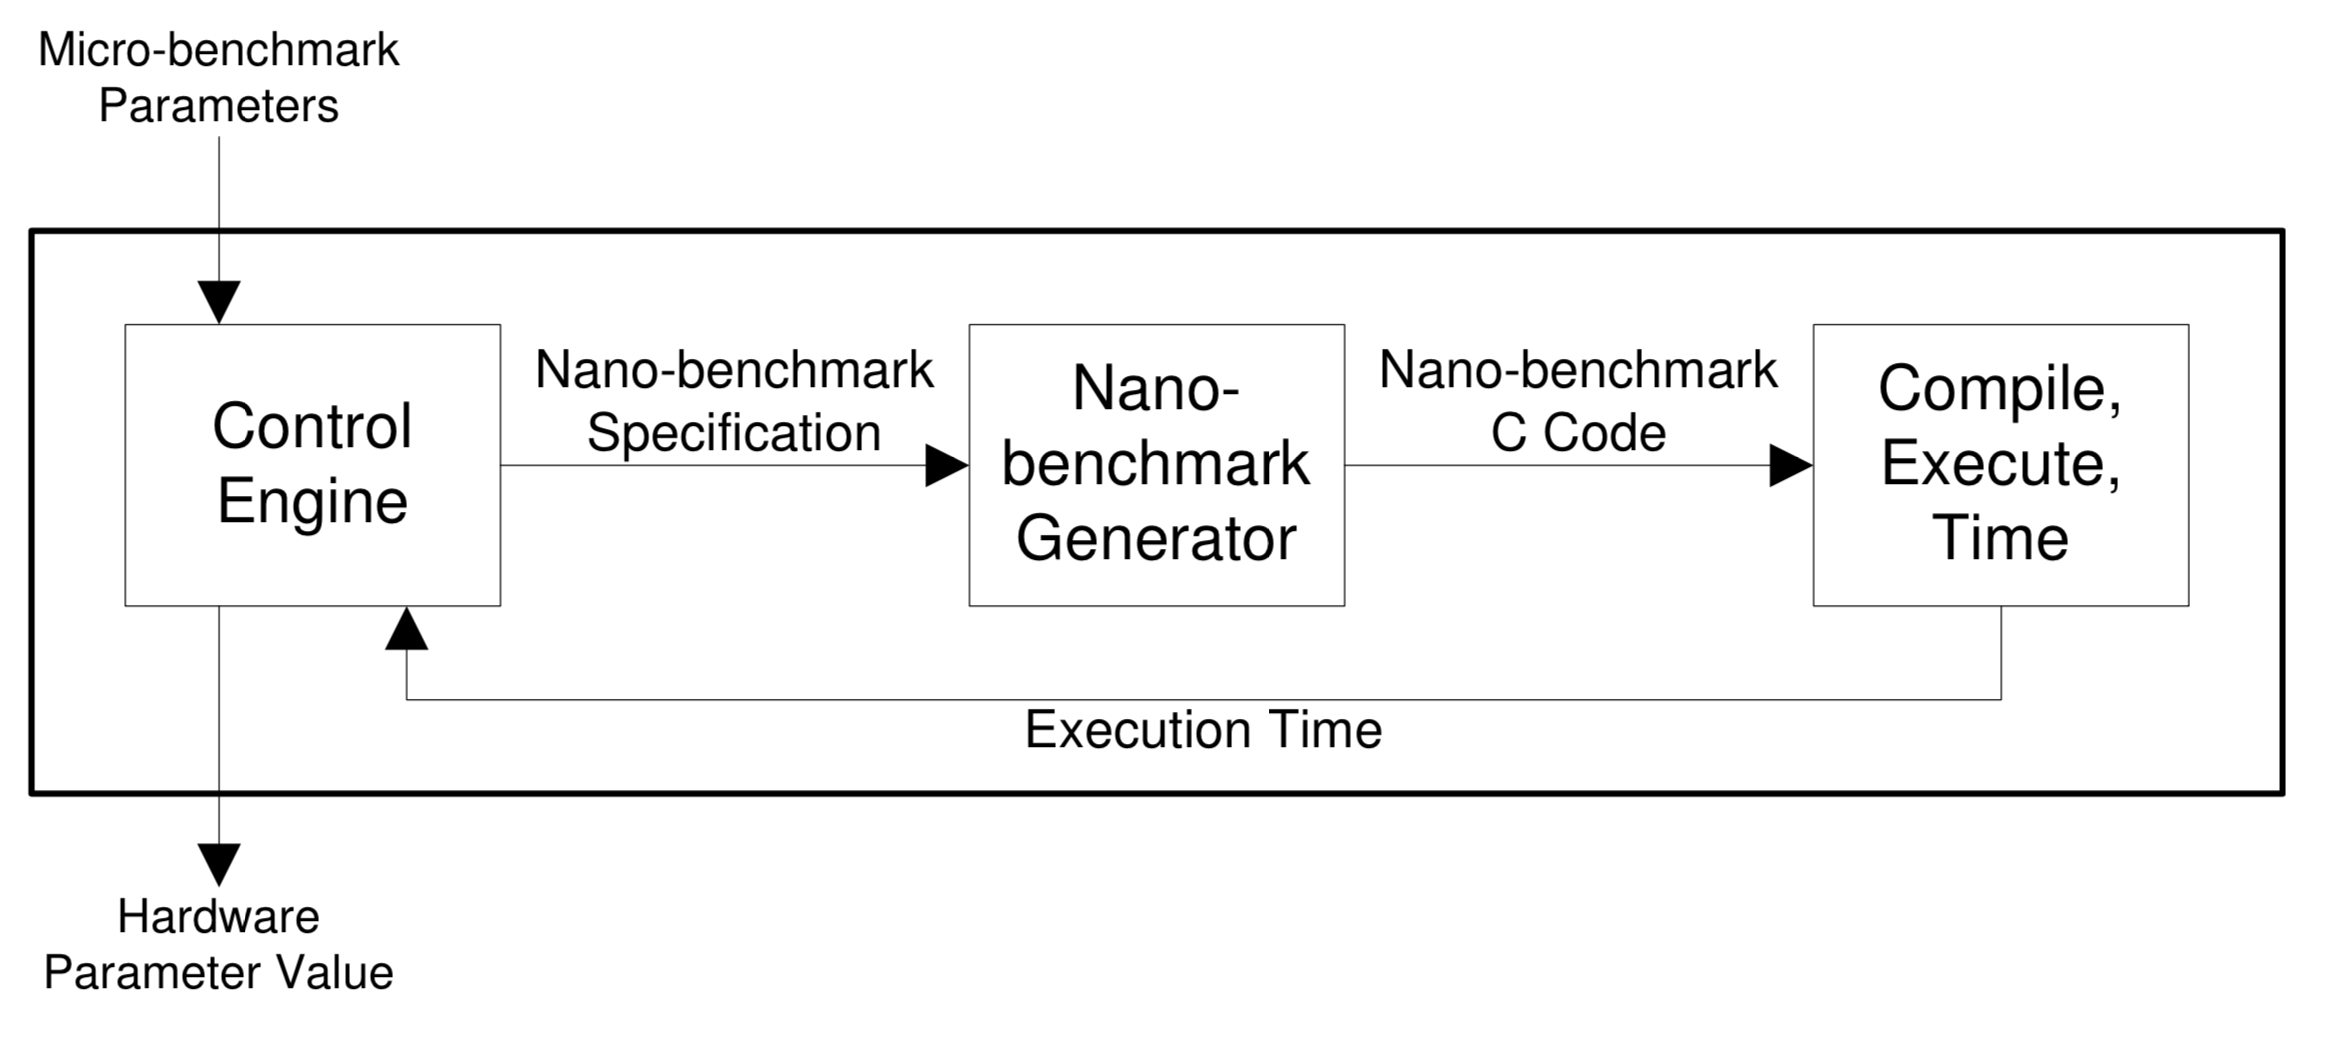
\includegraphics[width=10cm]{images/bench_xray.png}
                \caption{ Structure d'un micro benchmark réalisé grâce à X-Ray  \cite{Yotov2004}.
                \label{pic_bench_xray}}
            \end{figure}
            
             Le travail \cite{Yotov2005} utilise X-Ray pour implémenter des micros benchmarks pour mesurer la capacité, l'associativité, la taille des blocs ainsi que la latence de chaque niveau de la hiérarchie de caches ainsi que du TLB. Contrairement aux benchmarks existants, l'outil mesure un niveau à la fois, lui permettant d'être plus précis que les approches traditionnelles (X-Ray, Calibrator, lmbench et MOB). Utiliser X-Ray pour implémenter leur benchmark leur permet de mesurer la fréquence du processeur ainsi que la latence et le débit des instructions. Malheureusement, le code de X-Ray n'a pas été maintenu et n'est plus disponible au téléchargement.
        
        \paragraph{P-Ray \cite{Duchateau2008}.} 
        
             
            Pour remédier à l'incapacité de \textit{lmbench} à caractériser les plateformes multicoeurs, le benchmark P-ray a été développé. Pour cela il étend les micros benchmarks existant pour trouver le niveau des caches partagé, la topologie d’interconnexion, la bande passante effective ou la taille des blocs pour la gestion de cohérence des caches. Pour éviter les optimisations du compilateur (\textit{pointer chaising}), le benchmark utilise un système de liste chaînée lors de l'initialisation. Les résultats obtenus sont eux très précis et s'approchent souvent des maximums théoriques attendus.

            Dans le but de permettre à certaines librairies (ATLAS, SPIRAL ou FFTW) de s'auto-optimiser, P-Ray permet de mesurer certains paramètres matériels. De la même façon que X-Ray et LMbench, l'apport de P-Ray permet de trouver ces spécifications pour des processeurs multicoeurs. P-Ray permet de décrire la répartition des caches entre les coeurs, la topologie d'interconnexion des processeurs ainsi que les mécanismes de cohérence de cache. Leurs expérimentations montrent des résultats très précis comme la mesure de la latence de communication entre deux coeurs à travers le cache L3 ou entre deux processeurs. Un effort particulier a été apporté pour éviter des optimisations du compilateur et du préchargment mémoire (\textit{memory prefetcher}) pouvant altérer les performances mesurées. Le benchmark P-Ray a hérité d'un problème de X-Ray rendant impossible la portabilité du code entre différents systèmes d'exploitation. L'allocation mémoire suppose que toutes les adresses physiques soient contiguës et cette caractéristique dépend du système d'exploitation (les pages larges pouvant ne pas être disponibles). Le code de P-Ray n'est cependant pas libre de droits.
        
        \paragraph{Servet \cite{gonzalez2010servet}.} 
            La suite Servet permet de mesurer certaines caractéristiques des matériels, telles que la hiérarchie de cache (taille, partage entre les coeurs) ou la bande passante mémoire. Ce travail complète X-Ray et P-Ray par des mesures de paramètres d'interconnexion pour la communication d'une mémoire distribuée ainsi qu'une méthodologie et une nouvelle technique de mesure \textbf{todo reprendre cette phrase}. Une suite de benchmarks permet aussi d'évaluer où se formeront les goulots d'étranglement lorsque plusieurs coeurs accèdent à la mémoire centrale. Enfin, Servet mesure la distance entre les coeurs en mesurant la latence de communication permettant à une application de placer plus efficacement les processus sur les différents coeurs.
               
        \paragraph{Saavedra \cite{Saavedra1995}} 
        
            Ce benchmark utilise une \gsl{stride} (un saut en mémoire) de taille fixe pour accéder aux éléments d'un tableau. Le temps nécessaire à ces accès permet de déduire la taille des niveaux de la hiérarchie. Les expérimentations utilisent des couples de $\{taille de tableau, taille de stride\}$. La taille du tableau augmente jusqu'à atteindre la taille du cache mesuré. La taille des strides est limitée à des tailles de puissance de 2 et ne dépassera jamais la taille du cache. Le tableau est ainsi parcouru pendant au moins une seconde. Comme le souligne \cite{Yotov2005} le problème d'une telle approche est de vouloir mesurer tous les niveaux de la hiérarchie simultanément. Les mesures peuvent alors être influencées par différents paramètres de différents niveaux de caches. Ces mesures doivent être interprétées par l'utilisateur, le programme ne créant pas automatiquement la hiérarchie. La lecture et l'écriture sont réalisées sur la même donnée pouvant introduire des conflits dans le tampon d'écriture  \cite{Yotov2005}. Le benchmark suppose que les données sont continues en mémoire, mais n'utilise pas de pages larges.

       
\subsection{Analyse de performance d'une application}\label{sec:profiling}
%%%%%%%%%%%%%%%%%%%%%%%%%%%%%%%%%%%%%%%%%%%%%%%%%%%%%%%%%%%%%%%%%%%%%%%%
%%%%%%%%%%%%%%%%%%%%%%%%%%%%%%%%%%%%%%%%%%%%%%%%%%%%%%%%%%%%%%%%%%%%%%%%

        Le suivi de performances (\textit{performance monitoring}) a pour but de récolter des informations concernant une application ou concernant le système sur lequel elle est exécutée, pour la déboguer ou l'optimiser. L'analyse de performance peut être réalisée à différents niveaux \cite{imbert2011tips} : 
        \begin{itemize}
            \item Le premier niveau concerne l'utilisation d'un simulateur permettant d'étudier précisément (cycle par cycle) le comportement d'une architecture. Les données collectées peuvent être riches et permettent d'apporter des informations qu'il ne serait pas possible d'avoir avec l'exécution réelle de l'architecture. L'avantage de cette méthode est de pouvoir réaliser des premiers tests, sans avoir accès à l'architecture. Ces simulations peuvent modéliser la totalité de la microarchitecture et suivre l'exécution d'une application. Cependant, cette méthode nécessite le développement de simulateurs complexes que seul le constructeur peut développer. Les simulations précises (au cycle près) sont lentes (quelques centaines de cycles simulés par seconde) et génère de grandes quantités de données difficiles à analyser \cite{palomares2015combining}. Pour y remédier, des simulateurs plus simples utilisant des traces générées sur une architecture réelle peuvent être utilisés \cite{Cmelik1995}. Les traces sont collectées lors d'une première exécution sur une architecture et sont rejouées dans un simulateur pour être étudiées.
            
            \item Le second niveau correspond à l'analyse de la performance d'un serveur (coeur, processeur, système mémoire, réseaux). L'analyse de performance peut consister à vérifier la bonne répartition du travail entre les processeurs et la bonne utilisation des coeurs. Certains problèmes de performance peuvent venir de la mauvaise utilisation des mémoires caches ou de celle du bus mémoire. Au niveau le plus fin, l'analyse de la performance des coeurs peut être difficile, car elle nécessite l'utilisation d'outils précis. La complexité de la microarchitecture rend d'autant plus difficile cette analyse, de solides connaissances sont nécessaires pour pouvoir les analyser. Suite à cette analyse, diverses optimisations peuvent être nécessaires: préchargement de la mémoire, utilisation d'instructions vectorielles, amélioration de la gestion de la localité des données (\autoref{sec:locality})... Les informations utilisées pour l'analyse peuvent être obtenues en instrumentant le code (manuellement ou grâce au compilateur) ou en récupérant certaines informations de l'architecture (compteurs matériels).
            
            \item Le dernier niveau concerne l'analyse de la performance du supercalculateur complet. Il peut s'agir de vérifier la bonne utilisation de la programmation distribuée et la répartition du travail entre les noeuds. Les supercalculateurs \gls{exascale} devront être hétérogènes. Il est donc capital que l'ordonnanceur de tâche (\textit{job scheduler}) place efficacement les différents processus.
        
        \end{itemize}
        
        Pour parvenir à extraire la performance des supercalculateurs, l'analyse et l'optimisation des applications doivent être faites aux trois niveaux. Ce travail de thèse s'intéresse à l'analyse de performance du second niveau. Afin de permettre l'analyse, le portage et l'optimisation des codes, deux étapes principales sont étudiées:
        \begin{enumerate}
            
            \item \textbf{Identifier les hot spots.} En 1971, Donald Knuth affirmait que la majorité de l’exécution d'une application se déroulait dans une fraction des lignes de codes \cite{knuth1971empirical}. Cette affirmation est aussi connue sous le nom de principe de Pareto  (règle du 80/20). Ce principe empirique postule que 80\% des effets sont le produit de 20\% des causes. Dans le domaine de l’analyse de performance, cela signifie que 20\% des lignes de code sont responsable de 80\% du temps de l'exécution de l'application. Ces zones de codes sont appelées points chauds ou \glspl{hotspot}. Cela est d’autant plus vrai pour les applications de calcul haute performance où la proportion de code responsable d'une grande partie de la performance peut être encore plus faible. Il est facile de comprendre que c'est l'optimisation de ces zones de codes qui aura le plus d'impact sur l'amélioration de la performance de l'application. Il est donc nécessaire de pouvoir identifier et caractériser ces zones.
            
            \item \textbf{Identifier les goulots d'étranglement.} Une fois les zones de codes prenant une part majeure dans le temps d'exécution de l'application, il est nécessaire de quantifier leur performance pour trois raisons: 
            \begin{itemize}
                \item La première est de mesurer l'écart entre la performance réelle de l'application et la performance théorique atteignable par l'architecture pour quantifier les opportunités d'optimisations. 
                \item La deuxième est de pouvoir identifier les raisons et les parties de la microarchitecture qui sont responsables de cette performance. 
                \item La troisième est de permettre de caractériser leurs besoins: latence et débit mémoire, calcul, stockage...
            \end{itemize}
            Pour pouvoir comparer la différence entre la performance théorique et celle mesurée lors de l'exécution de l'application, il est courant d'utiliser des modèles de performances. Ces modèles prennent en compte les caractéristiques techniques d'une microarchitecture (FLOPS, débit mémoire...) ainsi que celles de l'application. L'utilisation de tels modèles permet ensuite de savoir quand le travail d'optimisation est terminé (performance maximale atteinte) ou de prédire la performance de la même application sur un système différent.
        \end{enumerate}
        
         Afin de répondre aux besoins exprimés ci-dessus, la suite de cette section présente les différentes méthodes et les outils existants qui permettent de suivre la performance d'une application. Nous présentons ensuite un modèle simple permettant de quantifier les performances mesurées d'une application.
           
      
 
    \subsubsection{Analyse statique et dynamique}
    %%%%%%%%%%%%%%%%%%%%%%%%%%%%%%%%%%%%%%%%%%%%%%%%%%%%%%%%%%%%%%%%%%%    
        
        Afin d'obtenir les informations nécessaires pour l'analyse de la performance d'une application, deux approches peuvent être employées: l'analyse statique et l'analyse dynamique.
        
        \paragraph{L'analyse statique}
            
            L’analyse statique consiste à obtenir des informations sur une application sans avoir à l'exécuter. Cette analyse peut permettre de détecter des bogues \cite{Lattner2016} ou de modéliser la performance de l'application grâce à l'utilisation de modèles analytiques. L'analyse peut être réalisée à partir du code source, ou des instructions assembleur générées par le compilateur \cite{Djoudi2005, wong2015vp3}. L'utilisation de l'assembleur permet de valider le bon fonctionnement du compilateur \cite{charif2014cqa}, mais rend plus difficile la corrélation avec le code source \cite{de2010new}.
            
            Des outils existent et permettent de réaliser des analyses statiques d'applications. 
            Intel propose différents outils tel que Intel Architecture Code Analyzer (IACA) \cite{Hirsh2012} qui permet de réaliser une analyse statique d'un code grâce à l'ajout de marqueur dans le code source. Il permet, pour un noyau identifié, de détecter la présence de dépendance entre plusieurs itérations de boucle et de donner une estimation des performances (débit d'instructions, saturation des ports de l'ALU...). Cependant, il est nécessaire d'avoir identifié les zones de \textit{hot spots} pour les annoter, et il ne fonctionne que pour des architectures Intel. Le projet a été abandonné en avril 2019\footnote{Intel IACA - \url{https://software.intel.com/en-us/articles/intel-architecture-code-analyzer}}.
        
            L’outil Modular Assembly Quality Analyzer and Optimizer (MAQAO) \cite{Djoudi2005} permet de désassembler un binaire pour en extraire le code assembleur et de lister les fonctions et les boucles importantes de l’application. Il peut ensuite faire un retour à l’utilisateur sur la qualité de son code et lui donner des conseils pour l’améliorer. Il permet d'analyser différents points, dont les 4 présentés dans \cite{popov:tel-01412638} :
            \begin{itemize}
                \item La pression appliquée par les instructions sur les différents ports du processeur pour en déterminer le bottleneck.
                \item La performance crête d'un code (qui suppose que toutes les données sont disponibles dans le premier niveau de cache).
                \item L’intensité arithmétique en mesurant le rapport du nombre d’instructions réalisant des opérations sur des nombres flottants et le nombre nombre total d’instructions à exécuter.
                \item Le ratio de vectorisation en mesurant le rapport du nombre d’instruction utilisant la vectorisation sur le nombre d’instructions pouvant potentiellement l’être.
            \end{itemize}
                      
            L'analyse statique ne nécessite pas l'exécution de l'application pour être réalisée. Ceci est très avantageux pour analyser les applications \gls{hpc} dont l'exécution peut durer plusieurs heures. Malheureusement, l'absence d'exécution ne permet pas de détecter les nombreux problèmes de performances dus à la complexité de l'architecture. Il est donc très difficile d'anticiper la performance réelle des applications. 
                 
        \paragraph{L'analyse dynamique}
            
            Contrairement à l'analyse statique, l'analyse dynamique nécessite l'exécution de l'application pour évaluer sa performance. Elle permet d’apporter de nombreuses informations impossibles à avoir grâce à l’analyse statique. Les informations peuvent être obtenues grâce à l'implémentation matérielle de registres permettant de suivre l'activité de la microarchitecture. Ces registres peuvent être simples (temps écoulé) ou complexes (nombre d'instructions vectorielles exécutées). Il y a deux façons d'utiliser ces compteurs: le comptage et l'échantillonnage.
               
            \begin{itemize}
                \item La première méthode consiste à \textbf{compter} le nombre d'évènements arrivant entre deux intervalles de temps. Pour cela, le compteur est initialisé à $0$ et lu au bout d'une certaine période de temps. Les valeurs ainsi récupérées permettent de mesurer le nombre d'occurrences de ces évènements. Cette méthode est efficace, mais elle ne permet pas de connaître la partie du code responsable d'un évènement. Les ratios d'évènements, tels que les instructions exécutées par cycle, les taux de \textit{miss} de mémoire cache et les taux d'erreurs de prévision des branches, peuvent être calculés en divisant le nombre par le temps écoulé.
                
                \item La deuxième méthode consiste à \textbf{échantillonner} ces informations. Ce mode consiste à déclencher une interruption tous les $n$ évènements et sauvegarder certaines informations telles que le pointeur d'instruction. Pour cela, le registre de comptage est initialisé à la valeur $\text{MAX} - n$ ou $\text{MAX}$ correspond à la valeur maximale pouvant être stockée dans le registre. Lorsque $n$ évènements sont comptés, le registre déclenche un débordement (\textit{overflow}) et génère une exception traitée par le système d'exploitation. Grâce à un échantillonnage assez fin (nombre $n$ petit) et des méthodes de statistiques, il est possible d'approcher le nombre d'évènements généré par chaque instruction. La principale difficulté de cette technique est d'assurer suffisamment de précision lors de l'attribution d'un évènement à une instruction. En effet, entre le moment où l'interruption est générée et son traitement, plusieurs instructions peuvent avoir été exécutées. Des technologies telles que Intel PEBS\footnote{Documentation Intel - Intel 64 and IA-32 Architectures Software Developer's Manual Volume 3B, Chapter 18. \url{https://software.intel.com/sites/default/files/managed/7c/f1/253669-sdm-vol-3b.pdf}} (Processor Event-Based Sampling) ou AMD IBS (Instruction Based Sampling) \cite{Drongowski2007} agrémentent le processeur d'un tampon lui permettant de stocker les informations nécessaires. L'autre avantage de cette technologie est de réduire l'impact sur les performances dû au traitement individuel de chaque échantillon par le système d'exploitation. La PMU possède un tampon pouvant stocker plusieurs échantillons et n'interrompt l'exécution que lorsque ce tampon est plein. Le principal désavantage de cette technologie est le nombre restreint d'évènements compatibles. De plus, elle n'est pas compatible avec toutes les architectures réduisant la portabilité des outils l'utilisant.
            \end{itemize}
                
            %Certaines études \cite{Moseley2011} proposent d'abandonner les compteurs matériels au profit d'outils seulement logiciel comme Pin tool d'Intel \cite{RobertD.2011} ou Dyninst \cite{RobertD.2011, Laurenzano2012}. Le challenge n'est plus alors de récupérer les données qui peuvent être fait à faible impact (moins de 1\% grâce à des techniques de \textit{shadow profiling} ou \textit{brusty tracing} \cite{Moseley2011}), mais plutôt dans l'analyse de ces traces. L'utilisation de techniques d'apprentissages peut alors être une bonne piste pour valoriser ces données.  \cite{Moseley2011} explore des pistes où ces collections et analyses de traces seraient la clef. Les traces collectées par les clients seraient alors envoyées au constructeur pour les analyser et simuler de potentielles performances sur des architectures qui n'existent pas encore. Cela simplifierait les échanges avec les clients qui sont souvent réticents à sortir les jeux de données de leur centre.


    \subsubsection{Les compteurs matériels}
    %%%%%%%%%%%%%%%%%%%%%%%%%%%%%%%%%%%%%%%%%%%%%%%%%%%%%%%%%%%%%%%%%%%    
 
        Afin de fournir des informations pour permettre l'analyse de performance dynamique, la microarchitecture possède des registres spéciaux qui sont incrémentés lors du déclenchement d'un évènement. Ces registres sont appelés compteurs matériels et leur origine est expliquée dans l'\aref{annexe:hc}. Les évènements mesurés peuvent être matériels (cycle d'horloge, exécution d'une instruction, manque dans un cache...) ou logiciels (faute de page, changement de contexte...). Suivre l'évolution de ces compteurs peut alors être utilisé pour des raisons multiples \cite{Moseley2011} : optimisation guidée par profile \cite{Cavazos2006}, optimisation dynamique \cite{Dai2005}, adaptation de la gestion de l'énergie \cite{Isci2005}, ordonnancement des \textit{threads} pour les ressources partagées \cite{Moseley2006} et autres \cite{Shye2005, Shye2008}.
        
        L'avantage des compteurs matériels est d'être implémentés directement par le processeur sans quoi il serait impossible de suivre précisément l'activité de la microarchitecture (\textit{miss} dans les caches, remplacement dans la TLB, nombre de cycles exécutés). Il faudrait pour cela utiliser des simulateurs dont les résultats sont souvent différents des performances réelles des processeurs réels. La tâche du programmeur est de configurer les compteurs et consulter leur valeur pour réaliser son étude. Cependant l'utilisation des compteurs matériels a plusieurs inconvénients:
        \begin{itemize}
        
            \item \textbf{Programmation des compteurs}: Afin de pouvoir utiliser les compteurs, le programmeur doit connaître leur adresse et être capable d'encoder les évènements pour pouvoir les programmer. Ces informations sont disponibles dans les documentations fournies par les constructeurs de processeur et ne sont pas toujours complètes (ou protégées par des accords de non-divulgation). Le programmeur doit ensuite développer un code de bas niveau pour programmer individuellement chaque compteur. Nous montrons dans la \autoref{sec:perf_asm_msr} comment ceci peut être réalisé et démontrons la difficulté d'utiliser ces compteurs.
            
            \item \textbf{Validation des évènements}: Pour pouvoir tirer des conclusions des résultats mesurés par les compteurs, il est nécessaire de réaliser deux validations: la première est de s'assurer que l'évènement utilisé mesure bien le comportement souhaité, la deuxième est de valider le bon comportement du compteur matériel. Les évènements disponibles pour un processeur peuvent varier entre deux versions de processeurs rendant le développement d'outil très difficile. Intel propose la liste des évènements compatibles avec chaque architecture \footnote{Liste des évènements compatibles par architecture Intel - \url{https://download.01.org/perfmon/index/}}.
            
            \item \textbf{Interprétation des résultats}: L'interprétation des mesures obtenues est une difficulté majeure dans l'utilisation des compteurs matériels. Interpréter un évènement comme le ``\textit{nombre de miss par cycle dans le cache L1}'' est loin d'être trivial. Il faut être capable de définir un seuil au-delà duquel la valeur obtenue indique une mauvaise performance. Associer des \textit{bonnes} et \textit{mauvaises} valeurs aux évènements est un challenge \cite{Moseley2011}.
            
        \end{itemize}
        
    

        \paragraph{Choix d'un sous-ensemble d'évènements.} 
        
            Les avantages et les inconvénients résumés ici étaient pour la majorité déjà actuels en 2002 \cite{sprunt2002basics}. Ce domaine ayant peu évolué depuis toutes ces années, nous devons nous satisfaire de l'état actuel de ces technologies sans espérer d'amélioration. Les outils développés dans le cadre de cette thèse ont pour objectif d'être utilisés sur des architectures très différentes. Pour cette raison, nous avons décidé de restreindre le nombre d'évènements nécessaires pour leur fonctionnement et nous privilégions l'utilisation de compteurs accessibles sur la majorité des plateformes. Ces compteurs sont généralement les plus simples et les plus robustes: nombre de cycle et nombre d'instructions exécutées. Grâce à ces deux compteurs, le nombre d'instructions exécutées par cycle peut être calculé (IPC). Ce ratio est une donnée primordiale pour s'assurer de la performance d'un code, mais elle n'est pas suffisante. Un axe central de notre méthodologie de caractérisation des applications nécessite de pouvoir suivre l'activité du bus mémoire. Les compteurs permettant de compter distinctement les accès en lecture et écriture réalisés par chaque contrôleur mémoire sont alors nécessaires.
            L'expérience acquise durant ces travaux de thèse nous a montré que ce sous-ensemble d'évènements était suffisant pour poursuivre l'analyse de la performance d'une grande majorité d'applications.     

    
    \subsubsection{Interface pour utiliser les compteurs matériels} \label{sec:edl_monitoring_tools}
    %%%%%%%%%%%%%%%%%%%%%%%%%%%%%%%%%%%%%%%%%%%%%%%%%%%%%%%%%%%%%%%%%%%
        
        La totalité des supercalculateurs HPC utilise un système d'exploitation basé sur le noyau Linux. Nous nous intéressons dans cette partie aux différents moyens disponibles lors de l'écriture de cette thèse pour utiliser les compteurs qui sont compatibles avec cet environnement. Dans l'\aref{annexe:hardware_counter} nous présentons les différentes façons de programmer les compteurs:
        \begin{itemize}
            \item Instructions assembleurs \verb|wrmsr|, \verb|rdmsr| et \verb|rdpmc| (\autoref{sec:perf_asm_msr})
            \item Interface \verb|/sys| (\autoref{annexe:hc_sys})
            \item Commande \verb|lspci| et \verb|setpci| (\autoref{annexe:hc_lspci})
            \item Mappage de l'espace mémoire PCI (\autoref{annexe:hc_pcimap})
        \end{itemize}
 
        Ces méthodes nécessitent de solides connaissances de l'architecture étudiée. De plus, le code développé est très dépendant de l'architecture et rend difficile le développement d'outils sophistiqués et leur maintien sur différentes versions d'architectures. Afin d'absoudre l'utilisateur de ces difficultés, des interfaces plus hauts niveaux ont été développées. La suite de cette section présente ces différentes interfaces (voir \autoref{fig:edl_perf_arbre}).
            
            \begin{figure}[h]
            \center
            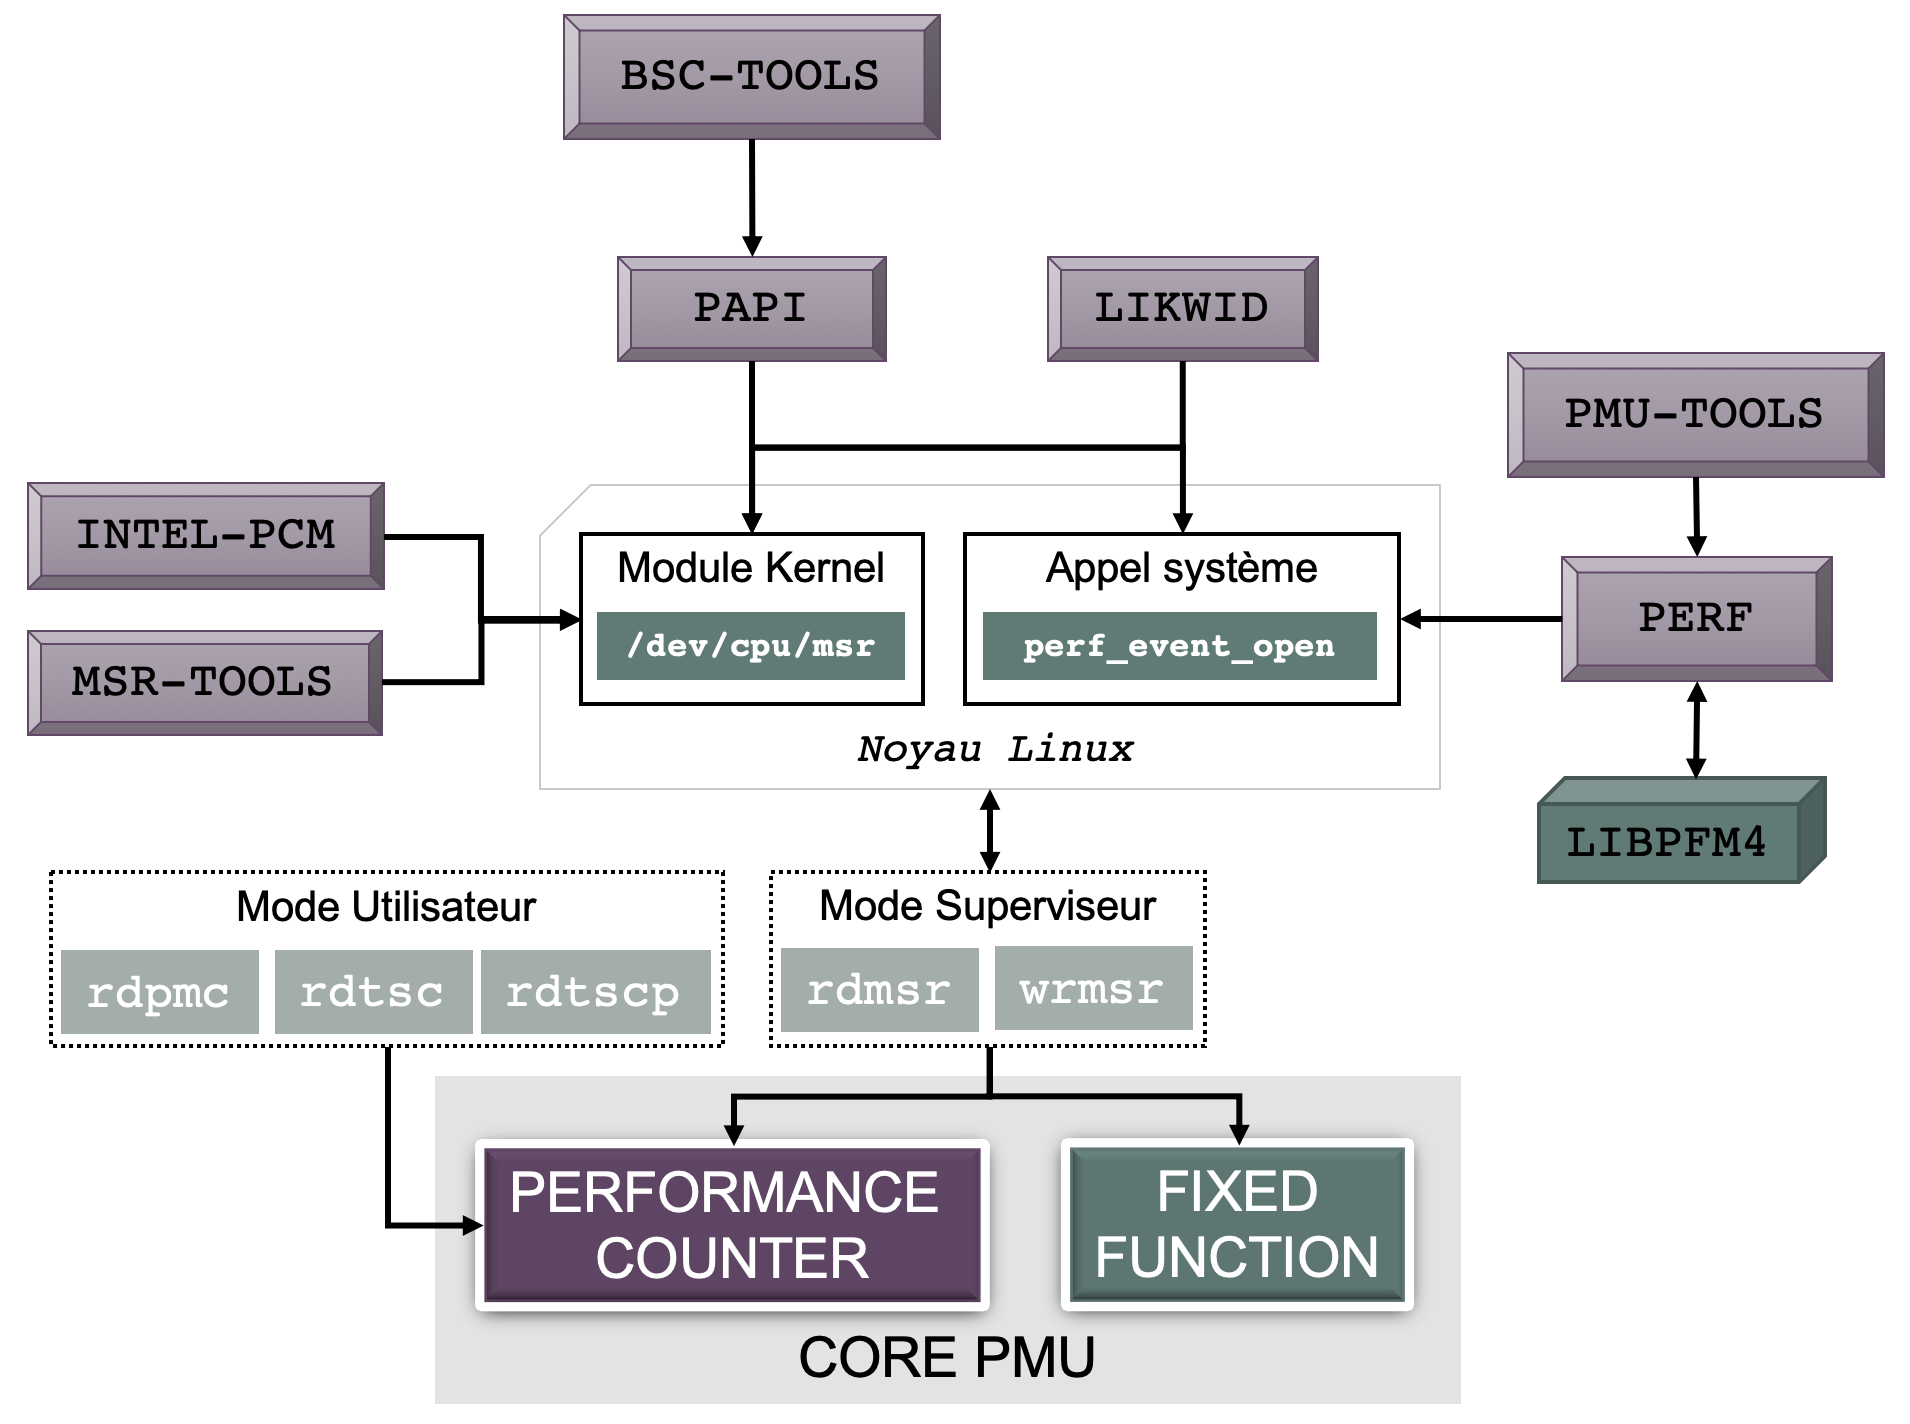
\includegraphics[width=14cm]{images/edl_perf_arbre.png}
            \caption{\label{fig:edl_perf_arbre} Différents moyens d'accéder aux compteurs localisés sur la PMU des coeurs. Linux propose deux interfaces permettant d'utiliser les deux instructions \textit{rdmsr} et \textit{wrmsr}: un module noyau et un appel système.}
            \end{figure}
           
        \paragraph{Perfmon2}
        %%%%%%%%%%%%%%%%%%%%%%%%%%%%%%%%%%        %%%%%%%%%%%%%%%%%%%%%%%%%%%%%%%%%%
            Le support par Linux des compteurs matériels a été long, empêchant les développeurs de construire des outils facilement portables. Pour ce faire, différents \textit{patchs} logiciels devaient être appliqués au noyau pour supporter leur utilisation. Nous pouvons citer \textit{perfctr} \cite{Pettersson2005} ou les projets \textit{perfmon} et \textit{perfmon2} \cite{Eranian2006}, développés par Stéphane Eranian, ancien employé HP. Le projet \textit{perfmon2} était le principal candidat à l'inclusion dans le noyau Linux avant l'émergence de \textit{Perf Events}. L'objectif du projet \textit{perfmon2} est de concevoir une interface générique de suivi des performances de bas niveau pour accéder à toutes les implémentations d'unités de surveillance des performances matérielles (PMU).
            L'interface utilise l'appel système \textit{perfmonctl}. Un appel système a été préféré à un driver de périphérique, car il offre une plus grande flexibilité et facilite la prise en charge par les implémentations d'un mode de surveillance par thread qui nécessite d'enregistrer et de restaurer l'état PMU du \textit{thread} \textbf{todo reference au glossaire}. L'interface exporte tous les registres PMU comme des registres 64 bits, même si de nombreuses implémentations de PMU en ont moins. L'interface ne sait pas ce que fait chaque registre, leur nombre, ni comment ils sont associés les uns aux autres. Toutes les informations spécifiques à un événement sont reléguées au niveau de l'utilisateur où elles peuvent être facilement encapsulées dans une bibliothèque.
        
            Le code de \textit{perfmon2} n'a jamais réussi à être inclus dans le projet Linux et son développement a été arrêté suite à la présentation du projet concurrent \textit{Performance Counters for Linux} (PCL) rebaptisé depuis \textit{Perf Events}.

        \paragraph{Perf Events}\label{sec:edl_profiling_perf}
        %%%%%%%%%%%%%%%%%%%%%%%%%%%%%%%%%%        %%%%%%%%%%%%%%%%%%%%%%%%%%%%%%%%%%
        
            Le projet de Compteur de Performance pour Linux (PCL) a été présenté en décembre 2008 et introduit dans Linux 2.6.31. Cet outil, rebaptisé \textit{Perf Events}, est une réponse au projet principal de standardisation des compteurs pour Linux de l'époque: perfmon2. Alors que ce dernier présentait beaucoup de fonctionnalités intéressantes, il n'a jamais réussi à être inclus dans le projet Linux. Lorsque \textit{Perf Events} fût ajouté au noyau Linux, de nombreuses fonctionnalités manquaient, mais sont apparues depuis. Pour fonctionner, \textit{Perf Events} utilise son interface \textit{perf\_event} développée directement dans le code du noyau Linux. Son adoption dans le noyau a mis un frein aux développements d'autres interfaces telles que \textit{perfmon2} ou \textit{perfctr} qui nécessitait de patcher le noyau pour être utilisée.  Du projet \textit{perfmon2}, seule la librairie \textit{libpfm4} est encore active. Il s'agit d'une librairie qui permet de convertir les noms symboliques d'évènements PMU en leur encodage pour \textit{Perf Events} ou d'autre interface noyau (exemple de la \autoref{fig:edl_perf_libpfm4}). La librairie en elle-même ne mesure aucun évènement. Elle fournit aux développeurs une interface pour lister, encoder les évènements pour beaucoup de PMU (core et uncore). Un point de désaccord persistant entre \textit{Perf Events} et d'autres approches (telle que \textit{perfmon2}) est qu'il incorpore toutes les informations sur les compteurs et les événements dans le code du noyau lui-même, ajoutant ainsi une quantité significative de code descriptif au noyau. L'intégration de telles données dans le noyau peut causer des difficultés aux outils utilisateur pour prendre des décisions sur les événements qui peuvent être comptés simultanément et aux fournisseurs pour fournir des mises à jour sans avoir à patcher le noyau ou attendre de nouvelles versions du noyau. L'interface introduit un seul appel système comme point d'entrée (\textit{sys\_perf\_open}) qui renvoie un descripteur de fichier qui donne accès aux événements matériels. 
            
            \begin{figure}[h!]
            \center
            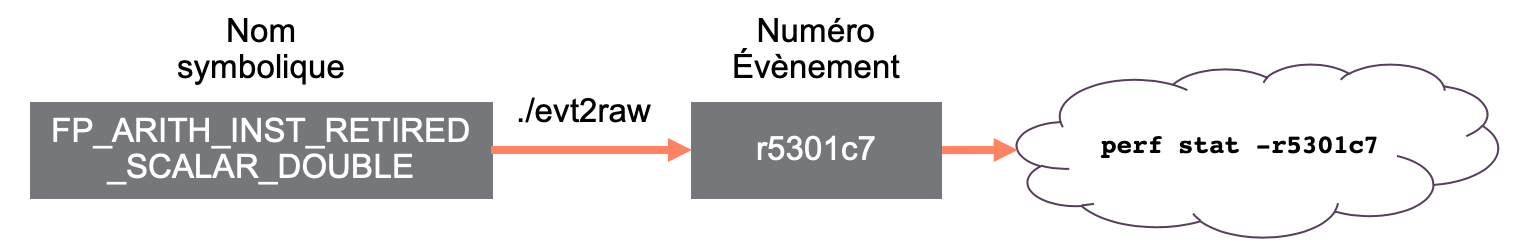
\includegraphics[width=12cm]{images/edl_perf_libpfm4.png}
            \caption{\label{fig:edl_perf_libpfm4} \textit{Libpfm4} permet de convertir les noms symboliques des évènements en leur encodage correspondant pouvant être utilisé avec des outils tels que \textit{perf}.}
            \end{figure}
 
        \paragraph{Pseudo système de fichier /dev/cpu/CPUID/msr}
        %%%%%%%%%%%%%%%%%%%%%%%%%%%%%%%%%%
            
            Linux permet à l'utilisateur un accès bas niveau aux MSR (registres matériels) sans avoir à utiliser de langages assembleurs. Ceci est réalisé à travers un pseudo système de fichier permettant d'interagir avec tous les coeurs (identifié par leur \verb|CPUID|) à travers le chemin \verb|/dev/cpu/#CPUID/msr|. Par défaut, seul l'utilisateur \textit{root} est autorisé à modifier ce fichier, mais ces droits peuvent être modifiés pour étendre l'accès aux autres utilisateurs. L'utilisation de cette interface est très pratique et peut être réalisée en accédant au fichier \textit{msr} grâce aux opérations \verb|pread()| et \verb|pwrite()|. Par exemple, pour lire le MSR dont l'adresse est \verb|0x38|, il suffit d'ouvrir le fichier \textit{msr} correspondant au coeur voulu, et réaliser une lecture avec un décalage de 38 octets. Pour faciliter l'usage de l'interface, Intel propose l'outil \textit{msr-tools} sur son GitHub\footnote{\url{https://github.com/intel/msr-tools}} (voir \autoref{fig:edl_perf_msrtools}).  La compilation produit deux exécutables \verb|rdmsr| et \verb|wrmsr| qui permettent de réaliser les lectures et écritures des registres MSR comme cela: \verb|./rdmsr -r 0x38D|. Nous proposons dans notre travail trois scripts permettant d'initialiser et configurer les compteurs grâce à ces deux programmes\footnote{\url{https://github.com/PourroyJean/performance_modelisation/tree/master/src/tool_PMU}}. 

            
            \begin{figure}[h!]
            \center
            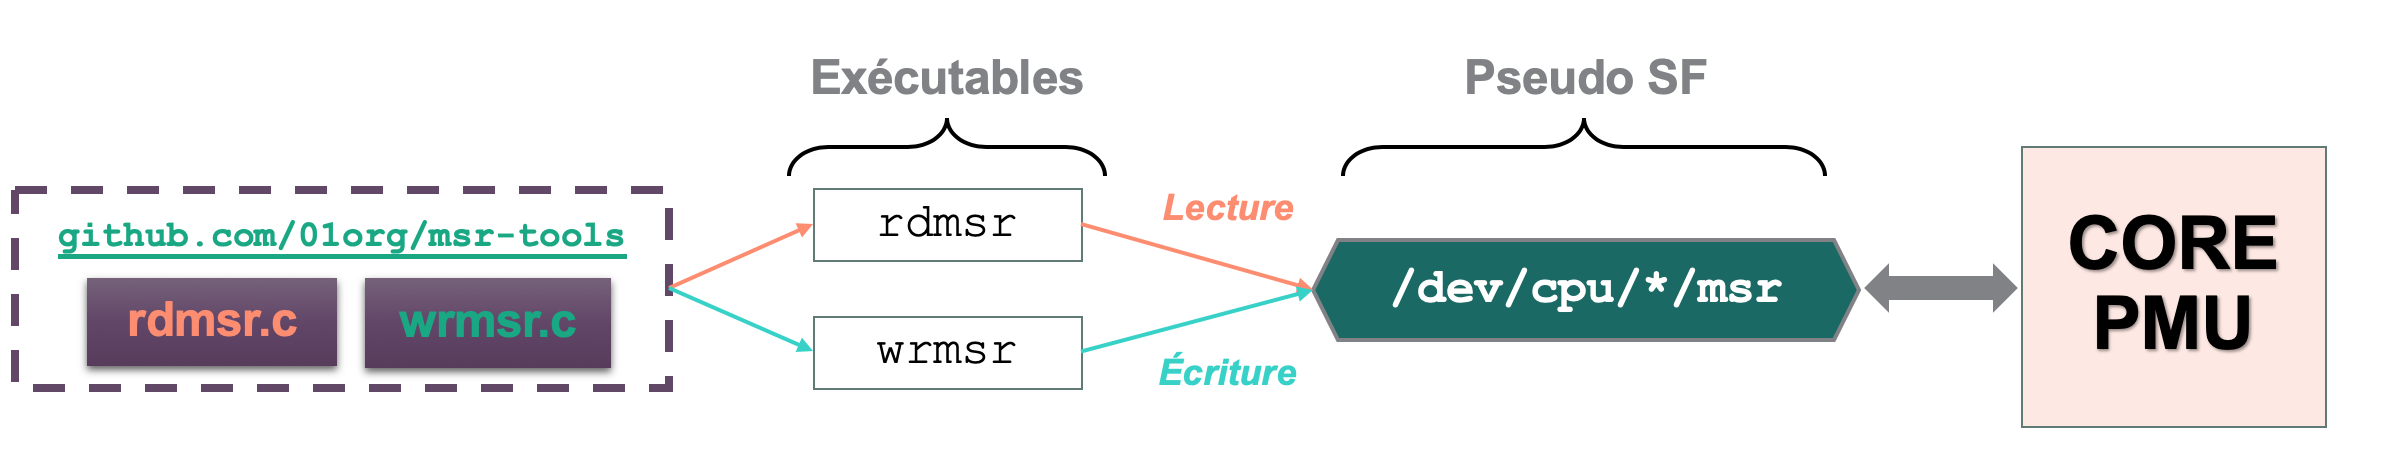
\includegraphics[width=16cm]{images/edl_perf_msrtools.png}
            \caption{\label{fig:edl_perf_msrtools} Intel propose deux exécutables permettant d'interagir plus facilement avec le pseudo système de fichier.}
            \end{figure}


    \subsubsection{Outils d'analyse de performance}
    %%%%%%%%%%%%%%%%%%%%%%%%%%%%%%%%%%%%%%%%%%%%%%%%%%%%%%%%%%%%%%%%%%%
    
        Les interfaces présentées précédemment permettent de faciliter l'accès et la programmation des compteurs matériels. À l'aide de ces interfaces, de nombreux outils de suivi de performance ont pu être développés. Dans cette section, nous présentons les principaux outils utilisés pouvant avoir une utilité dans le travail fixé au début de cette partie.

        \paragraph{perf \cite{Weaver2013}.} 
        %%%%%%%%%%%%%%%%%%%%%%%%%%%%%%%%%%        %%%%%%%%%%%%%%%%%%%%%%%%%%%%%%%%%%
            
            En plus de l'appel système, \textit{Perf Events} fournit un outil accessible depuis l'espace utilisateurs lui permettant de contrôler le profilage. Nommé \textit{perf}, ce programme utilise l'interface noyau pour réaliser des mesures soit en échantillonnage soit en comptage. Différentes commandes sont disponibles pour compter les évènements (\textit{stat}, \textit{record}, \textit{top}, \textit{bench}) et afficher les résultats (\textit{report}, \textit{annotate}). Grâce à la commande \textit{perf}, il est possible de compter les évènements en utilisant directement leur nom. La commande suivante peut être utilisée pour mesurer le nombre de transactions en lecture réalisées par un contrôleur mémoire. Il faut pour cela, vérifier que le noyau utilisé est capable d'accéder aux PMU uncore (première commande ci-dessous). Ensuite, il faut vérifier que le noyau supporte l'utilisation des noms d'évènements symboliques (deuxième commande ou \verb|perf list|). Enfin, la troisième commande permet de compter le nombre d'évènements.
            
\begin{verbatim}
# ls /sys/bus/event_source/devices/* | grep uncore_imc
uncore_imc_0 uncore_imc_1 uncore_imc_3 uncore_imc_4 uncore_imc_5

# ls /sys/bus/event_source/devices/uncore_imc_1/events/
cas_count_read  cas_count_read.scale  cas_count_read.unit clockticks ...         

# perf stat –a -e uncore_imc_0/cas_count_read/
\end{verbatim}
            
            Malheureusement, lorsque les évènements voulus ne sont pas supportés par le noyau, il est nécessaire de se reporter à la documentation de l'architecture. Perf (comme PAPI) est capable de configurer les compteurs grâce à leur encodage (numéro de l'évènement, masque de configuration). Dans notre exemple, l'évènement est le numéro $0x04$ associé au masque $0x03$. Lorsque l'évènement est supporté par le noyau, c'est cette valeur qui est stockée dans les fichiers listés ci-dessus (première commande). Pour réaliser le même comptage que précédemment, la deuxième commande ci-dessous peut être utilisée:

\begin{verbatim}
# cat /sys/bus/event_source/devices/uncore_imc_1/events/cas_count_read
event=0x04,umask=0x03

#perf stat -a -e "uncore_imc_0/event=0x04,umask=0x03/"
Performance counter stats for 'system wide':
4.94 MiB  uncore_imc_0/cas_count_read/
\end{verbatim}

    
           Le travail de Andy Kleen (\textit{pmu-tools}\footnote{pmu-tools: \url{https://github.com/andikleen/pmu-tools}}) peut aussi être utilisé pour faciliter l'utilisation de \verb=perf= lorsque les noms symboliques des évènements ne sont pas supportés. \verb=Ocperf= est un \textit{wrapper} de la commande \verb=perf= qui traduit les événements de la liste complète des événements Intel au format \textit{perf} lorsque ceux-ci ne sont pas supportés (première commande):

\begin{verbatim}
#perf  stat -e FP_ARITH_INST_RETIRED.128B_PACKED_DOUBLE sleep 1
invalid or unsupported event

#./ocperf.py  stat -e FP_ARITH_INST_RETIRED.128B_PACKED_DOUBLE sleep 1
perf stat –e cpu/event=0xc7,umask=0x4,name=fp_arith_inst_retired_128b_packed_double/ sleep 1
... correct ...
\end{verbatim}
        
        \paragraph{Oprofile \cite{Levon2004}.} 
        %%%%%%%%%%%%%%%%%%%%%%%%%%%%%%%%%%        %%%%%%%%%%%%%%%%%%%%%%%%%%%%%%%%%%
            
            Oprofile \cite{Levon2004} est un outil de suivi de performance développé par John Levon en 2001 dans le cadre de son projet de master et fut le principal outil de suivi de performance de Linux pendant plusieurs années\footnote{Source: \url{https://www.ibm.com/developerworks/linux/library/l-evaluatelinuxonpower/}}. 
            Oprofile est capable d'utiliser des compteurs de performances matérielles pour suivre la performance des processus, des bibliothèques partagées et du noyau. Pour suivre ces performances, Oprofile utilise un démon permettant à l'utilisateur de spécifier un événement matériel à surveiller et un seuil d'événement pour déclencher l'interruption (échantillonnage). En utilisant les tables de symboles de débogage, il peut faire le lien entre les adresses des instructions et les lignes du code source associées. Oprofile est un outil mature possédant une multitude d'options telle que la génération de graphiques d'appel (\textit{call graph}). Plusieurs utilitaires sont fournis à l'utilisateur pour contrôler le suivi de performance (\textit{opcontrol}, \textit{opreport} ...).
            À l'origine, Oprofile utilisait un module noyau nécessaire pour accéder aux PMU. Quand \textit{Perf Events} fut introduit avec son interface noyau, Oprofile a alors été adapté pour l'utiliser lui aussi. La communauté autour de la commande \verb|perf| est sans doute plus active et dynamique, et de nombreuses nouvelles fonctionnalités sont ajoutées à \textit{perf} sans analogies dans \textit{OProfile}.
 
        \paragraph{PAPI \cite{Browne2000}.}
        %%%%%%%%%%%%%%%%%%%%%%%%%%%%%%%%%%        %%%%%%%%%%%%%%%%%%%%%%%%%%%%%%%%%%
            
            L'interface Performance Application Programming Interface (PAPI), a pour objectif de simplifier l'utilisation des PMU de différentes architectures. Pour cela, PAPI offre une abstraction pour un grand nombre de compteurs d'évènements pour le développement d'outils de suivi de performance. Pour accéder aux MSR, PAPI utilisait l'interface \textit{perfctr} avant de basculer sur l'interface offerte par \textit{Perf Events} avec la version 2.6.32 du noyau Linux. PAPI supporte le comptage, l'échantillonnage ainsi que le multiplexage. Utiliser la totalité des fonctionnalités de PAPI nécessite une certaine expérience. Cependant pour un usage basique, son utilisation est très simple comme le montre l'exemple de l'\autoref{lst:edl_perf_pai}.

\begin{lstlisting}[
label=lst:edl_perf_pai,
basicstyle={\scriptsize\ttfamily},
identifierstyle={\color{black}},
language={c},
tabsize=2,
numbersep=8pt,
frame=tlbr,framesep=2pt,framerule=0pt,
morekeywords ={class,run},
caption=Utilisation simple de PAPI pour mesurer deux évènements dans un programme C.
]
#define NUM_EVENTS 2  
long_long values[NUM_EVENTS];
unsigned int Events[NUM_EVENTS]={PAPI_TOT_INS,PAPI_TOT_CYC};
PAPI_start_counters((int*)Events,NUM_EVENTS); /* Start the counters */
do_work();
PAPI_stop_counters(values,NUM_EVENTS); /* Stop counters and store results*/
\end{lstlisting}

        
            PAPI est composé de deux parties permettant de compter des évènements dits \textit{natifs} ou \textit{prédéfinis}:
            \begin{itemize}
                \item Les événements \textbf{natifs} comprennent l'ensemble des événements qui peuvent être comptés par le CPU. Dans de nombreux cas, ces événements seront disponibles par le biais d'un événement PAPI prédéfini correspondant. Il y a généralement beaucoup plus d'événements natifs disponibles qu'il n'est possible d'en faire correspondre sur des événements prédéfinis du PAPI. Même si aucun événement prédéfini n'est disponible, les événements natifs sont toujours accessibles directement. L'utilisation de ces évènements nécessite d'avoir une bonne connaissance de l'architecture utilisée. Chaque évènement peut être configuré grâce à un \textit{masque} pour désigner précisément l'évènement à compter de la même façon que lors de la programmation des MSR grâce aux commandes \textit{rdmsr} et \textit{wrmsr} présentées dans la \autoref{sec:perf_asm_msr}. 
            
                \item Les événements \textbf{prédéfinis} sont un ensemble commun d'événements jugés pertinents et utiles pour le réglage des performances des applications. Ces événements se trouvent généralement dans de nombreux CPU fournissant des compteurs de performance et donnent accès à la hiérarchie de la mémoire, aux événements du protocole de cohérence du cache, au nombre de cycles et d'instructions, à l'unité fonctionnelle et au statut du pipeline. En outre, les événements prédéfinis sont des correspondances de noms symboliques (nom prédéfini du PAPI) à des définitions spécifiques à la machine (événements natifs). Par exemple, le nombre total de cycles passés en mode utilisateur est PAPI\_TOT\_CYC\footnote{source:\url{https://icl.cs.utk.edu/projects/papi/wiki/Events}}. Un évènement prédéfini peut utiliser une combinaison d'un ou plusieurs évènements natifs. Par exemple, l'évènement permettant de complter le nombre de calculs flottants à simple précision réalisés, peut être mesuré avec l'événement prédéfini \textit{PAPI\_SP\_OPS}. Cet évènement utilise en réalité quatre évènements natifs pour compter les instructions vectorielles de différentes tailles pour ensuite calculer le résultat \textit{Number of FLOPS} (voir ci-dessous).
            \end{itemize}
            
            

\begin{verbatim}
#papi_avail -e PAPI_SP_OPS
    Number of Native Events:      4
    Long Description:            |Single prec. op; vector|
    Postfix Processing String:   |N0|N1|4|*|+|N2|8|*|+|N3|16|*|+||
    Number of FLOPS= N0 + N1 * 4 + N2 * 8 + N3 * 16
\end{verbatim}

            Il existe une centaine d'évènements prédéfinis par PAPI. La disponibilité de ces derniers peut être vérifiée grâce à la commande \verb|papi_avail|. Il est possible de créer ses propres jeux d'évènements prédéfinis. En raison des différences d'implémentation matérielle, il n'est pas toujours possible de comparer directement les comptes d'un événement prédéfini par PAPI obtenu sur différentes plates-formes matérielles.

        \paragraph{Likwid \cite{Treibig2010}.}
        %%%%%%%%%%%%%%%%%%%%%%%%%%%%%%%%%%        %%%%%%%%%%%%%%%%%%%%%%%%%%%%%%%%%%
        
            \textit{LIKWID} est un ensemble d'outils utilisables en ligne de commande pour aider les développeurs dans leur travail de caractérisation de plateformes et d'analyse de performances. Les outils fonctionnent sur la majorité des distributions Linux grâce à sa faible dépendance à des libraires externes: il ne nécessite que le compilateur \textit{GNU compiler}. L'outil possède 11 outils pouvant être groupés en trois catégories: analyse de performance, caractérisation de plateforme et contrôle de l'exécution. Deux outils sont importants pour analyser les performances d'une application: \textit{likwid-perfctr} et \textit{likwid-perfscope}.
        
            Le premier permet d'accéder aux compteurs de performances à travers les interfaces principales telles que \textit{Perf Events} ou \textit{perf\_ctr}. Les principaux évènements sont accessibles (\textit{core} et \textit{uncore}) et la majorité des processeurs x86 sont supportés grâce au sous-système \textit{perf\_event\_open()} (Intel Xeon, Intel Xeon Phi, et AMD Zen). L'avantage de cet outil est de pouvoir utiliser des groupes d'évènements déjà existants tels que:

\begin{lstlisting}
FLOPS_SP   Operation flottante simple precision MFlops/s
L3          Bande passante du cache L3 en MBytes/s
MEM         Bande passante mémoire en MBytes/s
\end{lstlisting}

            L'outil peut être utilisé pour mesurer la performance d'un système ou d'une application particulière utilisant la programmation multicoeur. 
        Likwid propose une API permettant d'annoter le code pour ne mesurer la performance que de certaines régions de l'application:
\begin{lstlisting}
LIKWID_MARKER_START(Compute);
<code>
LIKWID_MARKER_STOP(Compute);
\end{lstlisting}
            Pour pouvoir fonctionner, l'application doit être compilée avec le drapeau de compilation \verb|-DLIKWID_PERFMON|. L'avantage est de pouvoir facilement désactiver la mesure de performance et n'ajouter aucun coût supplémentaire à l'application lors d'une utilisation en production.
        
        
            Le deuxième outil, \textit{likwid-perfscope}, est un outil de visualisation des données mesurées par le premier. Il permet par exemple d'afficher l'évolution du trafic mémoire lors de l'exécution de l'application ou de la consommation énergétique. Malheureusement, cet outil n'est pas supporté pour les processeurs Skylake. Après avoir discuté avec le développeur de cette application, il semble que cet outil soit un "\textit{jouet}" et que le développeur originel ne fasse plus partie du projet.
            
           
        \paragraph{BSC Performance Tools}
        %%%%%%%%%%%%%%%%%%%%%%%%%%%%%%%%%%        %%%%%%%%%%%%%%%%%%%%%%%%%%%%%%%%%%
            Le centre de recherche du Barcelona Supercomputing Center développe depuis 1991 une suite d'outil permettant la caractérisation des applications. Cette suite d'outils est principalement composée de trois outils: \textit{Extrae} \cite{Rodriguez}, \textit{Paraver} \cite{Pillet1995} et \textit{Dymemas} \cite{Labarta1997}. La philosophie d'utilisation de ces outils est d'aider l'utilisateur à trouver le goulot d'étranglement \textbf{todo en gls} des performances de son application qui peut résulter de plusieurs causes. Les outils ne sont pas une boîte noire répondant à toutes les questions automatiquement. La méthodologie d'analyse, comprenant l'utilisation de \textit{Paraver} et \textit{Dimemas}, est basée sur l'examen de la distribution temporelle et spatiale des données de performance pour comprendre le comportement de l'application, détecter ses différentes phases et identifier la structure comportementale (qui peut être différente de la structure procédurale). Cette analyse détaillée permet d'extraire beaucoup d'informations des données de performance recueillies au cours de l'exécution. L'utilisateur doit être un programmeur confirmé dans l'analyse de performance et utiliser les outils pour l'aider dans son analyse de performance. Les outils permettent de facilement comparer plusieurs traces correspondant à différentes exécutions de l'application (paramètres ou architectures différents). 
            
            L'outil \textit{Extrae} signifie \textit{extraire}. Il permet notamment d'instrumenter dynamiquement un code pour en extraire des traces qui pourront être visualisées avec l'outil \textit{Paraver} (\textit{pour voir}). L'outil injecte une librairie (\verb=LD_PRELOAD=) pour annoter les différents symboles de l'application. La librairie \textit{Dyninst} est utilisée pour réaliser l'instrumentation au niveau du code source ou directement dans le fichier binaire. L'ensemble des outils est compatible avec \textit{OpenMP} et \textit{MPI} pour permettre d'obtenir des profils d'exécution parallèle. La \autoref{fig:edl_perf_paraver} montre un exemple de deux traces dont les graphiques sont alignés pour faciliter l'extraction de résultats. La première fenêtre montre en rouge les appels à des fonctions de communication de la librairie \textit{MPI}. Les parties en noir représentent le code de l'application propre à chaque coeur. La deuxième fenêtre montre à l'aide d'un dégradé de couleur le nombre d'instructions utiles par cycle. Les couleurs claires représentent un \textit{IPC} plus faible. On remarque ainsi que les communications ne sont pas parfaitement synchrones et que des coeurs perdent un certain temps à attendre que les autres coeurs aient fini leur partie du travail. L'outil \textit{Paraver} possède une visualisation sous forme de tableur permettant de quantifier le temps perdu à cause de ces désynchronisations et d'identifier le nom des fonctions responsables.  
        
            \begin{figure}
            \center
            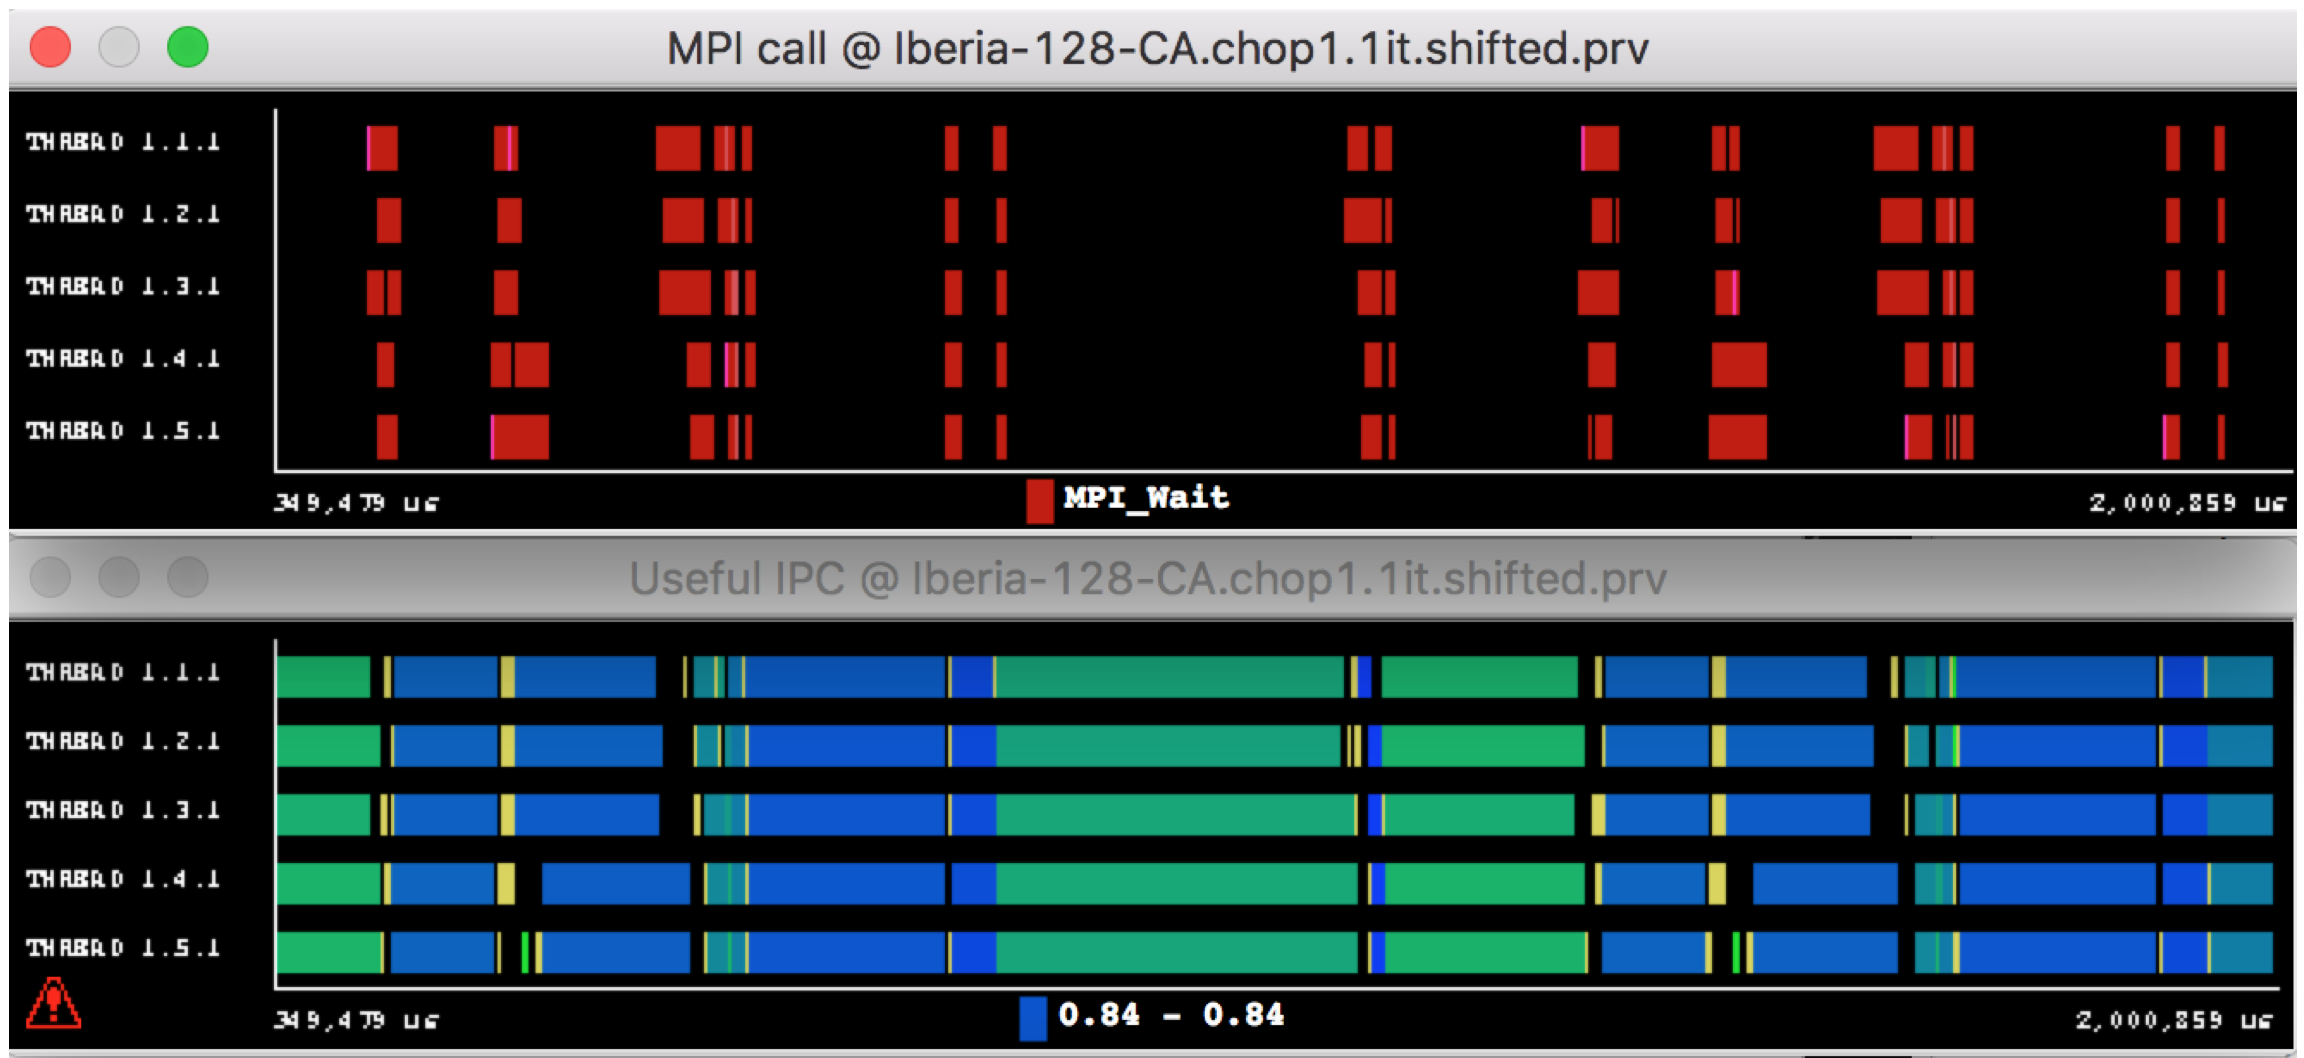
\includegraphics[width=12cm]{images/edl_perf_paraver.png}
            \caption{\label{fig:edl_perf_paraver} L'outil \textit{Paraver} permet d'afficher le graphique des traces obtenues grâce à l'outil \textit{Extrae}.}
            \end{figure}
            
            Le troisième outil, \textit{Dimemas}, permet à l'utilisateur de développer et optimiser des applications parallèles sur son poste de travail, tout en fournissant une prédiction précise de leurs performances sur une architecture parallèle. Le simulateur Dimemas reconstruit le comportement temporel d'une application parallèle sur une machine modélisée par un ensemble de paramètres de performance. Ainsi, les expériences de performance peuvent être faites facilement. L'absence de latence du réseau (virtuel) permet d'estimer les performances de son application si elle utilisait un supercalculateur avec un réseau parfait. L'utilisateur peut ensuite estimer l'impact apporté par le portage sur MPI et OpenMP. Les traces générées par \textit{Dimemas} peuvent ensuite être analysées avec l'outil \textit{Paraver}.


    \subsubsection{Modèle de performance: le Roofline model} \label{sec:roofline}
    %%%%%%%%%%%%%%%%%%%%%%%%%%%%%%%%%%%%%%%%%%%%%%%%%%%%%%%%%%%%%%%%%%%
        
        %\paragraph{Introduction}
        %    1. THESE - Preparing depth imaging applications for Exascale challenges and impacts .pdf
        %        - liste des modèles
    
            Présenté par William et al. en 2009 \cite{Williams2008}, le modèle du \textit{roofline} est un modèle de performance simple qui représente graphiquement les performances d’un code en situant sa performance par rapport aux performances maximales de l’architecture. L’objectif principal de ce modèle est de donner le pourcentage de la performance disponible atteinte par un code. L’intérêt de ce modèle est de restreindre l’analyse de performance aux deux ressources importantes pour les applications HPC: la performance calculatoire (GFLOPS) et la performance du bus mémoire (GB/s).
            Le modèle est utilisé pour représenter les différentes fonctions clefs d’une application. Ainsi, le programmeur pourra commencer son travail d’optimisation sur les fonctions avec le plus de potentiel.
            
            \begin{figure}
                \center
                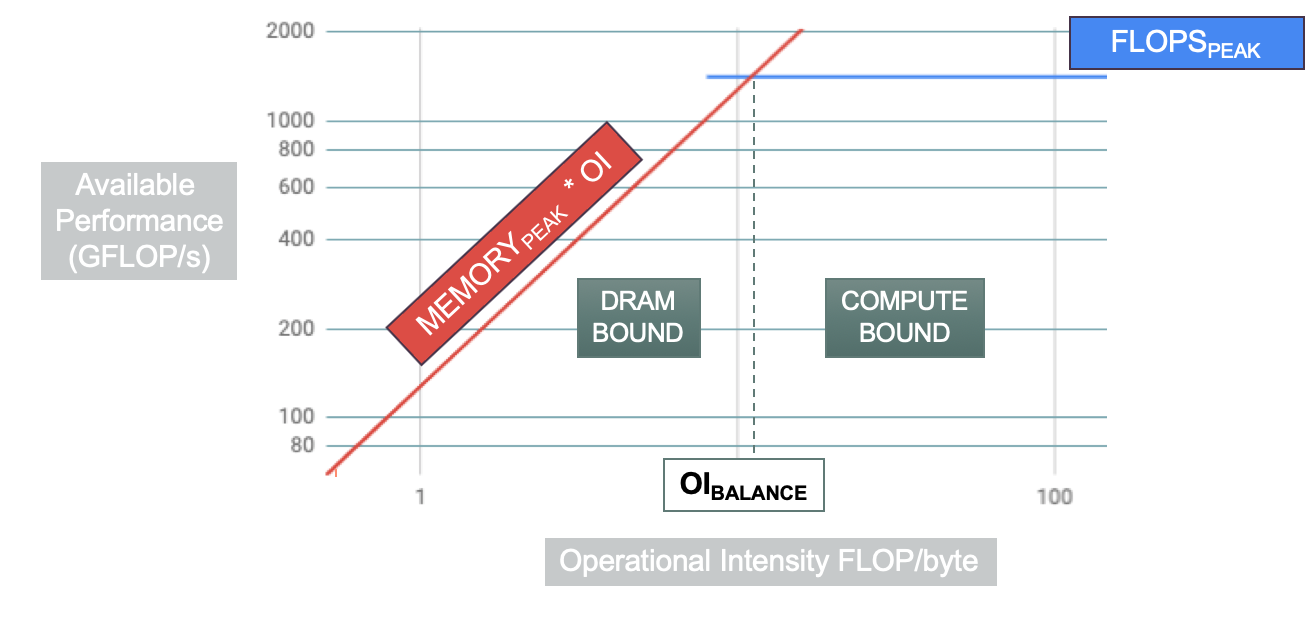
\includegraphics[width=12cm]{images/roofline.png}
                \caption{\label{fig:roofline} Représentation graphique du modèle du \textit{roofline}. En fonction de son intensité opérationnelle, la performance d'un code sera limitée par la bande passante ou par le processeur. \textbf{todo gls memory bound}}
            \end{figure}
            
            
            La \autoref{fig:roofline} montre une représentation du modèle du \textit{roofline}. Sur l’axe des abscisses est représentée l’intensité opérationnelle de l’algorithme (en FLOPS/byte) qui correspond au nombre d’opérations flottantes appliquées à chaque byte de donnée amené depuis la mémoire. Sur l’axe des ordonnées est représentée la performance de calcul mesurée en GFLOPS.
            Chaque \textit{hot spot} \textbf{todo gls} est placé en fonction de son intensité opérationnelle, calculée à partir de la lecture du code, et de sa performance, mesurée lors de l’exécution.
        
        \paragraph{Modélisation}
        %%%%%%%%%%%%%%%%%
            L’objectif du modèle est de déterminer si la performance du code pour une architecture donnée est structurellement limitée par la performance du processeur ($FLOPS_{peak}$ en $GFLOP/s$) ou bien par la performance du bus mémoire ($MEMORY_{peak}$ en $GB/s$). Une application réalisant la lecture de deux nombres pour y réaliser des centaines d’opérations verra ses performances limitées par la capacité de calcul $FLOPS_{peak}$ du processeur. Inversement, une application devant lire un grand jeu de données pour ne réaliser qu'une opération sur chaque valeur verra ses performances limitées par celle du bus mémoire $MEMORY_{peak}$. On peut estimer la quantité de calculs à réaliser sur chaque donnée en calculant son Intensité Opérationnelle  ($\text{OI}$ en $FLOP/byte$). Pour cela il faut lire le code source pour compter manuellement le nombre d’opérations réalisées ($\text{\#FLOP}$) et le nombre de données nécessaires chargées depuis la mémoire ($\text{\#BYTE}$). On peut ainsi calculer l’Intensité Opérationnelle d’un code en faisant le ratio des deux valeurs.
            
            \begin{equation}
            \begin{aligned}
                    \text{OI}_{kernel} =\ &\cfrac{\text{\#FLOP}}{\text{\#BYTE}}
            \end{aligned}
            \end{equation}
            
            Le temps pour exécuter le code ($\text{TEMPS}_{theorique}$), sera le temps mis par la ressource la plus utilisée par le code. On peut estimer ce temps par la formule suivante.
            \begin{equation}
            \begin{aligned}
                 \text{TEMPS}_{theorique} =\  &max 
                 \begin{cases} 
                    \quad \cfrac{\text{\#FLOP}}{\text{FLOPS}_{peak}}    \\[15pt]
                    \quad \cfrac{\text{\#BYTE}}{\text{MEMORY}_{peak}}
                \end{cases}
            \end{aligned}
            \end{equation}
            
            
            
            
            La performance théorique du code ($\text{PERF}_{theorique}$ en GFLOPS) peut être calculée grâce aux transformations successives de l'\autoref{eq:PERFT}.
            \begin{equation}
            \begin{aligned}
            \label{eq:PERFT}
            \cfrac{\text{TEMPS}_{theorique}}{\text{\#FLOP}}  =\ &\text{max}
            \begin{cases} 
                \cfrac {1}{\text{FLOPS\_{peak}}}    \\[15pt]  
                \cfrac {\cfrac{\text{\#BYTE}}{\text{MEMORY}_{peak}}}{\text{\#FLOP}} 
            \end{cases}\\[20pt]
            \cfrac{\text{\#FLOP}}{\text{TEMPS}_{theorique}}  =\ &\text{min}
            \begin{cases} 
                \text{FLOPS}_{peak}    \\[15pt]  
                \cfrac{\text{\#FLOP}}{\text{\#BYTE}} \times \text{MEMORY}_{peak}
            \end{cases}\\[20pt]
            \text{PERF}_{theorique}  =\ &\text{min}
            \begin{cases} 
                \text{FLOPS}_{peak}    \\[15pt]  
                \text{OI}_{kernel} \times \text{MEMORY}_{peak} 
            \end{cases}
            \end{aligned}
            \end{equation}
            
            2.13
                D'où
            2.14
                Considérant l'équation 2.11 on en déduit
            2.14
                
            Pour une architecture, il faut déterminer pour quelle intensité opérationnelle une application est limitée par la mémoire ou le processeur. Pour cela, il faut calculer l’intensité opérationnelle ($\text{OI}_{balance}$) correspondant au croisement des deux droites sur la \autoref{fig:roofline}. 
            
            \begin{equation}
            \begin{aligned}
             \text{FLOPS}_{peak} =\ &\text{OI}_{balance} \times \text{MEMORY}_{peak} \\[20pt]
             \text{OI}_{balance} =\ &\frac{\text{MEMORY}_{peak}} {\text{FLOPS}_{peak}} 
            \end{aligned}
            \end{equation}
            
            Une application dont l’intensité opérationnelle est inférieure à $\text{OI}_{balance}$ verra sa performance limitée par le système mémoire. Plus rarement, si l’intensité opérationnelle d’une application est supérieure à $\text{OI}_{balance}$, la performance sera alors limitée par le processeur.

        \paragraph{Construction}
        %%%%%%%%%%%%%%%%%%%%%%%%%%%%%%%%%%        %%%%%%%%%%%%%%%%%%%%%%%%%%%%%%%%%%

            La première étape dans la construction du graphique est de tracer les deux axes limitant les performances d’un code. Ces deux droites représentent les performances crêtes de la mémoire et du processeur. Pour obtenir ces valeurs, elles peuvent être calculées à partir des spécifications du processeur. Cependant, avec la complexification des architectures, il est difficile de les atteindre même avec des benchmarks prévus à cet effet. Il est donc préférable de les représenter par des valeurs mesurées comme indiqué dans la littérature  \cite{farjallah2014preparing}. Pour la mémoire, le benchmark STREAM peut être utilisé. Pour la performance du processeur, nous utilisons le générateur de benchmarks présenté dans la \autoref{sec:kg}. D’autres travaux sont venus compléter les benchmarks disponibles pour caractériser l’architecture \cite{lo2014roofline}.
        
        \paragraph{Évolutions}
        %%%%%%%%%%%%%%%%%%%%%%%%%%%%%%%%%%        %%%%%%%%%%%%%%%%%%%%%%%%%%%%%%%%%%

        
            Le \textit{roofine} a reçu de nombreuses améliorations depuis sa création. En 2014, les travaux \cite{Ilic2014} constate que le modèle original n’est pas suffisamment précis à cause de la faible précision de caractérisation de l’architecture. En effet, un code pouvant profiter de la localité des données dans les caches pourrait atteindre des performances supérieures au maximum prévu par le modèle utilisant seulement la bande passante mémoire. Inversement, la performance crête est calculée pour un code utilisant tous les coeurs du processeur, avec des instructions \gls{FMA} vectorisées. Cependant, par leur nature, certains codes ne peuvent pas utiliser ces  caractéristiques. La performance crête étant alors impossible à atteindre. Le modèle Cache-Aware Roofline Model (CARM) \cite{Ilic2014} a ainsi été développé permettant de représenter la performance des différents niveaux de caches. Cependant, le programmeur doit comprendre si son application peut profiter de cette localité, ce qui peut rendre cette approche plus difficile. Le modèle a depuis été affiné avec le Locality Aware Roofline Model (LARM) \cite{Denoyelle2018} permettant de modéliser les accès en mémoire non uniforme (NUMA).
            D’autres travaux essaient d’automatiser sa construction \cite{lo2014roofline} pour faciliter son usage. L’outil de profiling d’Intel a intégré les modèles CARM et LARM pour automatiser la recherche des hot spot et afficher leur performance sur un même graphique. Pour cela, il désassemble le code et calcule l’intensité opérationnelle de la boucle étudiée.

        \paragraph{Critiques}
        %%%%%%%%%%%%%%%%%%%%%%%%%%%%%%%%%%        %%%%%%%%%%%%%%%%%%%%%%%%%%%%%%%%%%

            
            La force de cette approche est de montrer rapidement au programmeur si son application est efficace ou non. Dans le cas échéant, il sait s’il doit travailler sur l’optimisation des FLOPS ou de la mémoire. En modélisant les principaux kernels \textbf{todo gls} de son application, le programmeur saura sur lesquels ses optimisations seront le plus bénéfiques.
            
            Bien qu'ayant reçu de nombreuses améliorations, ce modèle doit être utilisé pour commencer l’analyse de performance. Cependant, il ne permet pas de modéliser ni de comprendre finement la raison d’une performance.
            La majorité des applications étant limitée par la bande passante mémoire, il est rare d’utiliser ce modèle pour modéliser la performance des unités de calculs. Mais il peut être intéressant de calculer l’intensité opérationnelle d’une boucle pour s’en assurer avant d’apporter des optimisations. De plus, les accélérateurs à venir essaient de réduire le trou de performance entre les processeurs et la mémoire. Cette modélisation est donc importante pour l’analyse de performance.


\subsection{Conclusion} \label{sec:edl_hc_conclusion} \label{sec:edl_perf_conclusion}
%%%%%%%%%%%%%%%%%%%%%%%%%%%%%%%%%%%%%%%%%%%%%%%%%%%%%%%%%%%%%%%%%%%%%%%%
%%%%%%%%%%%%%%%%%%%%%%%%%%%%%%%%%%%%%%%%%%%%%%%%%%%%%%%%%%%%%%%%%%%%%%%%

    Dans cette section nous avons présenté les différentes méthodes et outils permettant de caractériser et de suivre les performances des architectures.  Nous avons présenté plusieurs des nombreux \glspl{benchmark} existants qui permettent de caractériser de nombreuses parties de la microarchitecture. Nous remarquons deux principaux manques concernant la caractérisation des unités arithmétiques et logiques et du système mémoire:
       \begin{itemize}
           \item Pour exécuter les instructions sur des nombres à virgule flottante, les ALU possèdent une unité de calcul spécialisée appelée FPU (\textit{floating point unit}). Sur un processeur moderne, la FPU est capable d'exécuter plusieurs instructions vectorielles par cycle (entre 1 et 4). L'expérience nous a montré que l'anticipation de ses performances était très difficile. Certaines particularités de cette unité (gestion des dépendances, exécution dans le désordre, fréquence soutenable) doivent être caractérisées pour aider à la compréhension de la performance d'une application. 
           
           \item Les applications \gls{HPC} utilisent couramment des accès mémoires réalisant des sauts entre deux adresses mémoires. Ces sauts (appelé \textit{stride}) peuvent être rencontrés dans de nombreux algorithmes. Par exemple, pour accéder à un champ appartenant à des objets stockés dans un tableau. L'adresse du champ des différents objets (dont la taille est constante) est séparée par un espace constant. L'accès au champ voulu des différents objets réalise donc des accès mémoire suivant un motif de saut. D’autres applications comme le calcul matriciel parcourent des matrices et génèrent des accès mémoire par saut de taille constante (taille d’une ligne de la matrice). Pour des tailles de sauts suffisamment grandes, l'accès suivant n'est pas présent dans la ligne de cache transférée lors de l'accès précédent. Afin d'obtenir des performances décentes, le pré chargeur de mémoire anticipe ces accès. La performance des applications dépend donc essentiellement de la capacité de ce matériel à comprendre le motif d'accès utilisé et les anticiper. Cependant, lorsque plusieurs jeux de données sont accédés simultanément, le préchargeur peut avoir des difficultés à les analyser. Ceci pouvant conduire à des performances désastreuses pour certaines applications clefs utilisées dans le HPC (algorithmes de stencil \cite{datta2008stencil}) Nous remarquons qu'aucun outil précédemment étudié ne permet d'évaluer cette fonctionnalité critique du matériel. 
       \end{itemize}
   
    
    Dans une seconde partie, nous avons présenté les différentes méthodes permettant d'accéder aux compteurs matériels. Ces compteurs permettent de suivre l'activité de la microarchitecture et d'aider à l'analyse de la performance d'une application. Nous avons pu discuter de la difficulté de programmer et des nombreux inconvénients qui accompagnaient leur utilisation. Les compteurs matériels n'ont en effet que peu évolué ces dernières années. Les évolutions de performance des processeurs ne nécessitaient pas d'investir des ressources et du temps dans l'analyse des performances. Les architectures se complexifiant de plus en plus, il est aujourd'hui très difficile d'expliquer la mauvaise performance d'un code. Le manque d'outil disponible et le besoin d'expertise rendent ce travail d'analyse très difficile. Afin d'accompagner le programmeur dans ce travail, nous proposons de contribuer à l'aide de deux développements:
    
    \begin{itemize}
        \item Le système mémoire est la ressource critique des architectures actuelles. Sa bonne utilisation étant primordiale, il est nécessaire de posséder un outil simple d'utilisation permettant de suivre son activité. 
        
        \item Afin de réaliser les optimisations les plus efficaces, il est nécessaire d'identifier les \textit{hot spots} d'une application. Il est alors nécessaire de disposer d'un outil permettant d'extraire ces zones de codes et de proposer une analyse simple au programmeur.
        
    \end{itemize}